% supplement_v2.tex -- the supplementary document of paper_v2 (B5, 25 November, as V1 and the
% Vietnamese version's N31 say): the former appendix of the paper (sections/appendix.tex, with tables
% t2, t3b, t5, t6, t8, t9 and figure f1), built as a document of its own. Its sections are lettered
% A-H and its tables and figure numbered S1, S2, ... Numbers without the S (Section 4, Table 3) are
% the paper's: they are read from paper_v2.aux with the xr package (labels prefixed P-), so the
% paper is built first. The latexmkrc in this folder does that on its own, also on Overleaf (Menu,
% Main document: supplement_v2.tex). The preamble is the paper's, copied: keep the two alike.
% Compile with pdfLaTeX and BibTeX, like the paper. It uses the same three .bib files.
\PassOptionsToPackage{dvipsnames}{xcolor}
\PassOptionsToPackage{obeyspaces,spaces}{url}   % \code keeps its spaces and can break at them
% nonacm: a draft not yet at an ACM venue, so no conference line, copyright block or ACM reference
% box. For a submission, drop nonacm and add the venue's settings.
\documentclass[sigconf,nonacm]{acmart}
\makeatletter
\@ACM@balancefalse   % no column balancing: acmart's \balance would come in the second column
\makeatother         % of the last page and only warn that it cannot balance there
\raggedbottom

\usepackage{array}
\usepackage{tabularx}
\usepackage{tikz}
\usetikzlibrary{arrows.meta,positioning}
\usepackage{pgfplots}
\pgfplotsset{compat=1.18}

\usepackage{xurl}   % long links may break anywhere in the narrow columns
% File names and meta-paths in typewriter type; they may break only after / _ . or at a space, so
% a meta-path such as PUPUP is never split.
\DeclareUrlCommand\codeurl{\def\UrlBreaks{\do\/\do\_\do\.}\def\UrlBigBreaks{}\urlstyle{tt}}
\DeclareRobustCommand{\code}[1]{\codeurl{#1}}
\newcolumntype{L}{>{\raggedright\arraybackslash}X}
\hyphenation{LMSPS}   % a name: never split as LM-SPS
% Wide tables and figures span both columns.
\newenvironment{widetable}[1][tbp]{\begin{table*}[#1]}{\end{table*}}
\newenvironment{widefigure}[1][tbp]{\begin{figure*}[#1]}{\end{figure*}}
% Figure colours, as in paper.tex: searched sets blue, manual orange, random draws aqua.
\definecolor{cSearch}{HTML}{2A78D6}
\definecolor{cManual}{HTML}{EB6834}
\definecolor{cRandom}{HTML}{1BAF7A}
\definecolor{cOther}{HTML}{7C7B76}
% Every number of the paper: \val{key}, from numbers.tex.
% numbers.tex -- written by make_numbers.py; do not edit by hand, run the script again.
% 2026-11-25: python make_numbers.py --lmsps LMSPS --han han-improve
% The raw-file counts come from extraction_report.json; the block below names the copy used.
% \val{key} prints a number; an unknown key prints ??key in bold and raises a LaTeX warning.
\makeatletter
\providecommand{\setval}[2]{\@namedef{val@#1}{#2}}
\DeclareRobustCommand{\val}[1]{\@ifundefined{val@#1}{\textbf{??#1}%
  \PackageWarning{numbers}{No value `#1' in numbers.tex}}{\@nameuse{val@#1}}}
\makeatother

% --- Data: the raw file, the fixes and the clean graph (LMSPS notes, Parts 2-4) ------------------
\setval{raw-records}{548,552}  % extraction_report.json (review/evidence/extraction_report.json)
\setval{raw-usable}{542,684}  % extraction_report.json (review/evidence/extraction_report.json)
\setval{raw-reviews}{7,593,244}  % extraction_report.json (review/evidence/extraction_report.json)
\setval{raw-categories}{49,732}  % extraction_report.json (review/evidence/extraction_report.json)
\setval{raw-pos-pct}{78.6}  % audit_before_fix.json: share of review lines rated 4 or 5
\setval{raw-unhelpful-pct}{1.35}  % positive reviews dropped as unhelpful (>= 5 votes, < 20% helpful)
\setval{placeholder-ids}{6}  % extraction_report.json (review/evidence/extraction_report.json)
\setval{placeholder-lines}{1,147,920}  % extraction_report.json (review/evidence/extraction_report.json)
\setval{placeholder-main-lines}{945,065}  % extraction_report.json (review/evidence/extraction_report.json): ATVPDKIKX0DER
\setval{placeholder-second-lines}{201,770}  % extraction_report.json (review/evidence/extraction_report.json): A3UN6WX5RRO2AG
\setval{edition-pairs}{64,814}  % extraction_report.json (review/evidence/extraction_report.json)
\setval{edition-clusters}{30,648}  % extraction_report.json (review/evidence/extraction_report.json)
\setval{edition-products}{72,280}  % extraction_report.json (review/evidence/extraction_report.json)
\setval{raw-works}{501,052}  % usable products after merging editions
\setval{kcore-iterations}{13}  % extraction_report.json (review/evidence/extraction_report.json)
\setval{catpath-rows}{2,288,922}  % extraction_report.json (review/evidence/extraction_report.json)
\setval{placeholder-main-max}{1,056}  % most reviews on one product
\setval{placeholder-second-max}{1,193}
\setval{placeholder-found}{4}  % IDs found by the rule, not named in advance
\setval{placeholder-found-max-lo}{57}  % their most reviews on one product
\setval{placeholder-found-max-hi}{149}
\setval{placeholder-found-lines}{1,085}
\setval{edition-size-min}{2}  % products in an edition cluster
\setval{edition-size-max}{24}
\setval{edition-size-two-pct}{79.5}  % clusters of exactly two products
\setval{rule-pos-rating}{4}  % a positive review is rated at least this
\setval{rule-helpful-votes}{5}  % a review with at least this many votes ...
\setval{rule-helpful-pct}{20}  % ... and fewer helpful ones than this is dropped
\setval{rule-kcore}{5}
\setval{rule-edition-shared}{3}  % identical review lines two editions must share ...
\setval{rule-edition-overlap-pct}{50}  % ... covering this share of the smaller one
\setval{rule-edition-maxrun}{50}  % review lines on more products than this are ignored
\setval{rule-placeholder-repeats}{50}  % reviews on one product that mark a placeholder
\setval{before-products}{90,659}
\setval{before-categories}{39,754}
\setval{before-users}{171,285}
\setval{before-edges}{2,612,766}
\setval{before-maxdeg}{55,572}  % largest user degree
\setval{before-meddeg}{7}  % median user degree
\setval{before-clusters}{17,726}  % duplicate-edition clusters
\setval{before-clustered}{44,591}  % products in those clusters
\setval{before-clustered-pct}{49.2}
\setval{before-copyedges-pct}{55.0}  % edges that copy an interaction already in the graph
\setval{before-valleak-pct}{72.9}  % validation edges with a training copy
\setval{before-testleak-pct}{73.0}  % test edges with a training copy
\setval{before-valtitle-pct}{60.3}  % validation edges whose user has a training edge to a same-title product
\setval{before-testtitle-pct}{60.2}  % the same for test edges
\setval{before-alsobought}{188,257}  % distinct also-bought product pairs
\setval{after-products}{48,883}
\setval{after-categories}{37,411}
\setval{after-users}{53,569}
\setval{after-edges}{819,847}
\setval{after-maxdeg}{2,134}  % largest user degree
\setval{after-meddeg}{8}  % median user degree
\setval{after-clusters}{6}  % duplicate-edition clusters
\setval{after-clustered}{12}  % products in those clusters
\setval{after-clustered-pct}{0.025}
\setval{after-copyedges-pct}{0.007}  % edges that copy an interaction already in the graph
\setval{after-valleak-pct}{0.011}  % validation edges with a training copy
\setval{after-testleak-pct}{0.010}  % test edges with a training copy
\setval{after-valtitle-pct}{0.86}  % validation edges whose user has a training edge to a same-title product
\setval{after-testtitle-pct}{0.80}  % the same for test edges
\setval{after-alsobought}{87,901}  % distinct also-bought product pairs
\setval{after-zerocat-pct}{60.7}  % categories with an all-zero name vector
\setval{after-leafcats-med}{5}  % leaf categories per product
\setval{title-coverage-pct}{95.8}  % products with a non-zero title vector
\setval{title-dim}{256}
\setval{title-vocab}{12,699}
\setval{cat-vocab}{128}
\setval{user-bits}{8}
\setval{user-dim}{64}
\setval{rel-pp-rows}{121,075}  % also-bought rows per direction
\setval{rel-cc}{37,400}
\setval{rel-pc}{427,565}
\setval{rel-up}{819,847}

% --- The split (rebuilt as hgb/link_data.py builds it; checked against the fingerprint) ----------
\setval{split-train}{655,879}
\setval{split-val}{81,984}
\setval{split-test}{81,984}
\setval{split-seed}{1}
\setval{split-fingerprint}{c5f7bccbf61c1b0f}
\setval{split-negatives}{99}
\setval{train-deg-med}{6}  % training edges per user
\setval{train-deg-mean}{12.2}
\setval{train-deg-max}{1,745}
\setval{test-users}{33,222}  % users with at least one test edge
\setval{group-book}{23,754}
\setval{group-book-pct}{48.6}
\setval{test-book-pct}{41.0}  % share of test edges
\setval{group-dvd}{4,359}
\setval{group-dvd-pct}{8.9}
\setval{test-dvd-pct}{13.9}  % share of test edges
\setval{group-music}{16,436}
\setval{group-music-pct}{33.6}
\setval{test-music-pct}{33.8}  % share of test edges
\setval{group-video}{4,334}
\setval{group-video-pct}{8.9}
\setval{test-video-pct}{11.3}  % share of test edges
\setval{group-bookmusic-pct}{82.2}
\setval{test-bookmusic-pct}{74.8}  % books and music, share of test edges

% --- The graph: category links, near-empty paths and edition twins (audits, link.dat, HAN logs) ---
\setval{before-topuser-pct}{61}  % share of products the largest user had reviewed before the fix
\setval{raw-shared-pct}{68.7}  % raw review lines that also appear under another product
\setval{cat-all-median}{13}  % categories per product if every ancestor were linked
\setval{cat-all-largest-pct}{48.7}  % products in one category, every ancestor linked
\setval{cat-pcp-ratio}{20.7}  % P-C-P walks with every ancestor linked, over leaves only
\setval{pcp-isolated}{9}  % products whose leaf categories hold no other product
\setval{pccp-reach-train-pct}{27.7}  % training edges whose product PCCP links to another product
\setval{pccp-isolated-pct}{81.1}  % products PCCP links to no other product (full graph)
\setval{pccp-reach-book-pct}{2.2}  % share of Book products that PCCP links to another product
\setval{pccp-reach-dvd-pct}{90.1}  % share of DVD products that PCCP links to another product
\setval{pccp-reach-music-pct}{5.3}  % share of Music products that PCCP links to another product
\setval{pccp-reach-video-pct}{90.2}  % share of Video products that PCCP links to another product
\setval{empty-isolated-min-pct}{76.2}  % near-empty paths: products without a neighbour, HAN graphs
\setval{empty-isolated-max-pct}{81.1}
\setval{pccp-graph-isolated-pct}{81.1}  % PCCP in the HAN graph (pruning adds a few)
\setval{pcccp-graph-isolated}{0}
\setval{pcp-graph-isolated}{9}
\setval{pp-isolated-pct}{11.3}  % products without an also-bought partner
\setval{twin-products}{51}  % products with an identical reviewer set elsewhere
\setval{twin-groups}{23}
\setval{twin-edges}{497}
\setval{twin-val}{47}
\setval{twin-test}{40}
\setval{example-shared}{659}  % review lines a DVD and a VHS of one film share (review part 1)
\setval{example-lines}{660}

% --- The search: 30 runs per set size (LMSPS notes, Parts 1 and 5-9) -----------------------------
\setval{search-cands}{36}
\setval{search-pool}{10}
\setval{search-sets}{210}  % sets scored per run (10 choose 4 = 10 choose 6)
\setval{search-epochs}{150}
\setval{search-warmup}{15}
\setval{search-hops}{5}
\setval{search-hidden}{512}
\setval{search-batch}{10,000}
\setval{search-dropout}{0.5}
\setval{search-lr}{0.001}
\setval{search-tau-max}{8}
\setval{search-tau-min}{4}
\setval{search-delta}{0.010}
\setval{search-folds}{4}  % folds of training edges for the weight step
\setval{search-alr}{0.001}  % learning rate of the alpha step
\setval{search-weight-decay}{0}
\setval{search-input-drop}{0}
\setval{env-gpu}{RTX 4070 SUPER}  % the run records
\setval{env-gpu-mem}{12}  % GB, the card's specification
\setval{env-python}{3.9.25}
\setval{env-torch}{2.1.2}
\setval{env-cuda}{12.1}
\setval{env-dgl}{2.2.1}
\setval{env-numpy}{1.26.4}
\setval{search-runs}{30}
\setval{search-runs-total}{60}
\setval{search-cands-raw}{55}  % P...P paths of at most 5 hops before merging reversed pairs
\setval{search-epoch-s-4}{6.9}  % median seconds per training epoch
\setval{search-prop-s-4}{37}  % median seconds of feature propagation
\setval{search-run-min-4}{18}  % median minutes per run (epochs + propagation)
\setval{search-fleet-h-4}{9.0}  % GPU hours for the 30 runs
\setval{search-winners-4}{26}  % distinct winners among the 30 runs
\setval{search-delta-alt}{0.005}  % the second tolerance of the vote (sensitivity check)
\setval{search-tie-med-4}{60}  % median tie-group size (delta 0.010)
\setval{search-tie-min-4}{13}
\setval{search-tie-max-4}{87}
\setval{search-tie-seed1-4}{83}  % tie group of seed 1
\setval{search-noise-4}{0.0055}  % score noise of one set
\setval{search-agree-4}{\ensuremath{+0.68}}  % Spearman of two runs on shared sets
\setval{search-xnoise-4}{0.0050}  % gap of a winner re-scored in another run
\setval{search-vote-4}{16}  % distinct vote picks
\setval{search-null-med-4}{21}
\setval{search-null-lo-4}{17}  % 90% range, as reselect_fleet.py
\setval{search-null-hi-4}{26}
\setval{search-null-share-4}{3.0}  % null fleets with as few distinct picks
\setval{search-vote-alt-4}{20}  % distinct vote picks
\setval{search-null-med-alt-4}{26}
\setval{search-null-lo-alt-4}{23}  % 90% range, as reselect_fleet.py
\setval{search-null-hi-alt-4}{29}
\setval{search-null-share-alt-4}{0.0}  % null fleets with as few distinct picks
\setval{search-cons-count-4}{5}  % runs whose vote pick is the consensus
\setval{search-null-fleets}{200}  % shuffled-score fleets in the null
\setval{search-avg-sets-4}{333}  % sets scored in at least 5 runs
\setval{search-se-4}{0.0025}  % standard error of the best averaged set
\setval{search-window-4}{2}  % sets within one SE of the best averaged score
\setval{search-epoch-s-6}{8.1}  % median seconds per training epoch
\setval{search-prop-s-6}{36}  % median seconds of feature propagation
\setval{search-run-min-6}{21}  % median minutes per run (epochs + propagation)
\setval{search-fleet-h-6}{10.7}  % GPU hours for the 30 runs
\setval{search-winners-6}{30}  % distinct winners among the 30 runs
\setval{search-tie-med-6}{78}  % median tie-group size (delta 0.010)
\setval{search-tie-min-6}{50}
\setval{search-tie-max-6}{146}
\setval{search-tie-seed1-6}{72}  % tie group of seed 1
\setval{search-noise-6}{0.0068}  % score noise of one set
\setval{search-agree-6}{\ensuremath{+0.59}}  % Spearman of two runs on shared sets
\setval{search-xnoise-6}{0.0039}  % gap of a winner re-scored in another run
\setval{search-vote-6}{19}  % distinct vote picks
\setval{search-null-med-6}{22}
\setval{search-null-lo-6}{19}  % 90% range, as reselect_fleet.py
\setval{search-null-hi-6}{25}
\setval{search-null-share-6}{11.0}  % null fleets with as few distinct picks
\setval{search-vote-alt-6}{20}  % distinct vote picks
\setval{search-null-med-alt-6}{25}
\setval{search-null-lo-alt-6}{22}  % 90% range, as reselect_fleet.py
\setval{search-null-hi-alt-6}{28}
\setval{search-null-share-alt-6}{1.0}  % null fleets with as few distinct picks
\setval{search-cons-count-6}{5}  % runs whose vote pick is the consensus
\setval{search-avg-sets-6}{169}  % sets scored in at least 5 runs
\setval{search-se-6}{0.0030}  % standard error of the best averaged set
\setval{search-window-6}{32}  % sets within one SE of the best averaged score
\setval{pilot-sets}{210}  % sets scored in each same-seed pilot run, all identical
\setval{search-total-h}{20}  % GPU hours for all 60 runs (epochs + propagation)
\setval{rank-pupup-4}{3.6}  % mean alpha rank of PUPUP (1 = most preferred of 36)
\setval{rank-pupup-6}{3.6}  % mean alpha rank of PUPUP (1 = most preferred of 36)
\setval{rank-puppup-4}{2.8}  % mean alpha rank of PUPPUP (1 = most preferred of 36)
\setval{rank-puppup-6}{4.1}  % mean alpha rank of PUPPUP (1 = most preferred of 36)
\setval{rank-pup-4}{9.1}  % mean alpha rank of PUP (1 = most preferred of 36)
\setval{rank-pup-6}{10.2}  % mean alpha rank of PUP (1 = most preferred of 36)
\setval{rank-pcp-4}{26.6}  % mean alpha rank of PCP (1 = most preferred of 36)
\setval{rank-pcp-6}{28.7}  % mean alpha rank of PCP (1 = most preferred of 36)
\setval{rank-pcccp-4}{22.3}  % mean alpha rank of PCCCP (1 = most preferred of 36)
\setval{rank-pcccp-6}{21.8}  % mean alpha rank of PCCCP (1 = most preferred of 36)
\setval{rank-pcpcp-4}{24.5}  % mean alpha rank of PCPCP (1 = most preferred of 36)
\setval{rank-pcpcp-6}{27.5}  % mean alpha rank of PCPCP (1 = most preferred of 36)
\setval{rank-ppccpp-4}{14.9}  % mean alpha rank of PPCCPP (1 = most preferred of 36)
\setval{rank-ppccpp-6}{6.4}  % mean alpha rank of PPCCPP (1 = most preferred of 36)

% --- Settings: the commands in the seed-1 logs of M5 (HAN, metapath2vec) and of GAT --------------
\setval{han-set-topk}{20}  % --topk
\setval{han-set-hidden}{512}  % --hidden
\setval{han-set-num-heads}{8}  % --num-heads
\setval{han-set-feat-drop}{0.2}  % --feat-drop
\setval{han-set-attn-drop}{0.2}  % --attn-drop
\setval{han-set-lr}{0.001}  % --lr
\setval{han-set-weight-decay}{0}  % --weight-decay
\setval{han-set-batch-size}{100,000}  % --batch-size
\setval{han-set-stage}{150}  % --stage
\setval{han-set-patience}{10}  % --patience
\setval{han-set-min-delta}{0.0005}  % --min-delta
\setval{han-set-beta-warmup}{15}  % --beta-warmup
\setval{mtv-set-dim}{512}  % --dim
\setval{mtv-set-walks-per-node}{5}  % --walks-per-node
\setval{mtv-set-walk-length}{20}  % --walk-length
\setval{mtv-set-window}{3}  % --window
\setval{mtv-set-negatives}{5}  % --negatives
\setval{mtv-set-lr}{0.01}  % --lr
\setval{mtv-set-epochs}{10}  % --epochs
\setval{mtv-set-evals-per-epoch}{4}  % --evals-per-epoch
\setval{mtv-set-patience}{6}  % --patience
\setval{mtv-set-min-delta}{0.0005}  % --min-delta
\setval{mtv-set-batch-walks}{1,024}  % --batch-walks
\setval{gat-set-in-dim}{256}  % --in-dim
\setval{gat-set-hidden}{512}  % --hidden
\setval{gat-set-num-heads}{8}  % --num-heads
\setval{gat-set-layers}{2}  % --layers
\setval{gat-set-feat-drop}{0.2}  % --feat-drop
\setval{gat-set-attn-drop}{0.2}  % --attn-drop
\setval{gat-set-lr}{0.001}  % --lr
\setval{gat-set-weight-decay}{0}  % --weight-decay
\setval{gat-set-batch-size}{100,000}  % --batch-size
\setval{gat-set-stage}{150}  % --stage
\setval{gat-set-patience}{10}  % --patience
\setval{gat-set-min-delta}{0.0005}  % --min-delta
\setval{han-set-head-dim}{64}  % dimensions per attention head
\setval{han-set-sem-dim}{128}  % semantic attention vector (model print in the log)
\setval{han-set-in-dim}{260}  % product input features: LSA title vector and product group
\setval{han-set-semantic-tau}{1}  % softmax temperature

% --- Path sets (HAN repository, arch.py) ---------------------------------------------------------
\setval{runs-total}{68}  % result rows: every model, set and seed
\setval{sets-distinct-paths}{32}  % distinct paths over the 24 sets, all among the candidates
\setval{sets-size-min}{2}  % paths per set, over the 24 sets
\setval{sets-size-max}{6}
\setval{sets-hops-max}{5}  % longest path in the 24 sets, hops
\setval{perm-shuffles}{20,000}  % permutation tests of the Spearman correlations
\setval{set-m1}{PUP PCP}  % amazon_lp_manual_1
\setval{set-m1-n}{2}
\setval{set-m1-hops}{4}
\setval{set-m2}{PP PUP PCP}  % amazon_lp_manual_2
\setval{set-m2-n}{3}
\setval{set-m2-hops}{5}
\setval{set-m3}{PP PUP PPUP}  % amazon_lp_manual_3
\setval{set-m3-n}{3}
\setval{set-m3-hops}{6}
\setval{set-m4}{PCP PCCCP PCPCP}  % amazon_lp_manual_4
\setval{set-m4-n}{3}
\setval{set-m4-hops}{10}
\setval{set-m5}{PP PUP PCP PPUP}  % amazon_lp_manual_5
\setval{set-m5-n}{4}
\setval{set-m5-hops}{8}
\setval{set-m6}{PP PUP PCP PPUP PPP PCCCP}  % amazon_lp_manual_6
\setval{set-m6-n}{6}
\setval{set-m6-hops}{14}
\setval{set-m7}{PP PPP PUP PCP}  % amazon_lp_manual_7
\setval{set-m7-n}{4}
\setval{set-m7-hops}{7}
\setval{set-m8}{PUP PCP PUPUP PCPUP}  % amazon_lp_manual_8
\setval{set-m8-n}{4}
\setval{set-m8-hops}{12}
\setval{set-r4d1}{PCCPPP PCPPUP PPCCPP PPPPP}  % amazon_lp_rand4_d1
\setval{set-r4d1-n}{4}
\setval{set-r4d1-hops}{19}
\setval{set-r4d2}{PCCPCP PCCPP PCPCP PPUP}  % amazon_lp_rand4_d2
\setval{set-r4d2-n}{4}
\setval{set-r4d2-hops}{16}
\setval{set-r4d3}{PCCCP PP PPPPP PUPUP}  % amazon_lp_rand4_d3
\setval{set-r4d3-n}{4}
\setval{set-r4d3-hops}{13}
\setval{set-r4d4}{PCCP PCPPPP PUP PUPPUP}  % amazon_lp_rand4_d4
\setval{set-r4d4-n}{4}
\setval{set-r4d4-hops}{15}
\setval{set-r4d5}{PCCPPP PCPP PCPUPP PPP}  % amazon_lp_rand4_d5
\setval{set-r4d5-n}{4}
\setval{set-r4d5-hops}{15}
\setval{set-r6d1}{PCCCCP PCCCPP PCCPCP PCCPP PCPUP PPUPP}  % amazon_lp_rand6_d1
\setval{set-r6d1-n}{6}
\setval{set-r6d1-hops}{27}
\setval{set-r6d2}{PCCCP PCPPUP PCPUPP PPCPP PPP PPUP}  % amazon_lp_rand6_d2
\setval{set-r6d2-n}{6}
\setval{set-r6d2-hops}{23}
\setval{set-r6d3}{PCCPPP PCPPCP PCPUP PPCPPP PPPPPP PUPUP}  % amazon_lp_rand6_d3
\setval{set-r6d3-n}{6}
\setval{set-r6d3-hops}{28}
\setval{set-r6d4}{PCCPP PPCPPP PPP PPPPP PPPPUP PUPUP}  % amazon_lp_rand6_d4
\setval{set-r6d4-n}{6}
\setval{set-r6d4-hops}{24}
\setval{set-r6d5}{PCCPPP PCPPCP PCPUP PPCPUP PPPPPP PPPUP}  % amazon_lp_rand6_d5
\setval{set-r6d5-n}{6}
\setval{set-r6d5-hops}{28}
\setval{set-f4a1}{PCCPCP PPCCPP PPUPP PUPUP}  % amazon_lp_v3_f4_a1
\setval{set-f4a1-n}{4}
\setval{set-f4a1-hops}{18}
\setval{set-f4a2}{PCCPPP PPCCPP PPPUPP PUPUP}  % amazon_lp_v3_f4_a2
\setval{set-f4a2-n}{4}
\setval{set-f4a2-hops}{19}
\setval{set-f4c}{PCCPP PPUPP PUPPUP PUPUP}  % amazon_lp_v3_f4_c
\setval{set-f4c-n}{4}
\setval{set-f4c-hops}{17}
\setval{set-f6a1}{PCCP PCCPP PPCCPP PPUP PUPPUP PUPUP}  % amazon_lp_v3_f6_a1
\setval{set-f6a1-n}{6}
\setval{set-f6a1-hops}{24}
\setval{set-f6a2}{PCCP PCCPCP PPCCPP PPUP PUPPUP PUPUP}  % amazon_lp_v3_f6_a2
\setval{set-f6a2-n}{6}
\setval{set-f6a2-hops}{25}
\setval{set-f6c}{PCCP PCCPUP PPCCPP PPUPP PUPPUP PUPUP}  % amazon_lp_v3_f6_c
\setval{set-f6c-n}{6}
\setval{set-f6c-hops}{26}

% --- Every set at seed 1: HAN and metapath2vec (results.csv) -------------------------------------
\setval{han-m1-hit-s1}{0.635}
\setval{han-m1-ndcg-s1}{0.398}
\setval{han-m1-fhit-s1}{0.0169}
\setval{han-m1-fndcg-s1}{0.0082}
\setval{han-m1-frec-s1}{0.0305}
\setval{han-m1-val-s1}{0.3072}
\setval{han-m2-hit-s1}{0.650}
\setval{han-m2-ndcg-s1}{0.413}
\setval{han-m2-fhit-s1}{0.0192}
\setval{han-m2-fndcg-s1}{0.0093}
\setval{han-m2-frec-s1}{0.0337}
\setval{han-m2-val-s1}{0.2957}
\setval{han-m3-hit-s1}{0.648}
\setval{han-m3-ndcg-s1}{0.416}
\setval{han-m3-fhit-s1}{0.0203}
\setval{han-m3-fndcg-s1}{0.0102}
\setval{han-m3-frec-s1}{0.0382}
\setval{han-m3-val-s1}{0.2935}
\setval{han-m4-hit-s1}{0.619}
\setval{han-m4-ndcg-s1}{0.375}
\setval{han-m4-fhit-s1}{0.0121}
\setval{han-m4-fndcg-s1}{0.0058}
\setval{han-m4-frec-s1}{0.0244}
\setval{han-m4-val-s1}{0.3194}
\setval{han-m5-hit-s1}{0.665}
\setval{han-m5-ndcg-s1}{0.427}
\setval{han-m5-fhit-s1}{0.0216}
\setval{han-m5-fndcg-s1}{0.0106}
\setval{han-m5-frec-s1}{0.0388}
\setval{han-m5-val-s1}{0.2814}
\setval{han-m6-hit-s1}{0.692}
\setval{han-m6-ndcg-s1}{0.453}
\setval{han-m6-fhit-s1}{0.0257}
\setval{han-m6-fndcg-s1}{0.0128}
\setval{han-m6-frec-s1}{0.0462}
\setval{han-m6-val-s1}{0.2651}
\setval{han-m7-hit-s1}{0.670}
\setval{han-m7-ndcg-s1}{0.433}
\setval{han-m7-fhit-s1}{0.0228}
\setval{han-m7-fndcg-s1}{0.0114}
\setval{han-m7-frec-s1}{0.0423}
\setval{han-m7-val-s1}{0.2834}
\setval{han-m8-hit-s1}{0.663}
\setval{han-m8-ndcg-s1}{0.427}
\setval{han-m8-fhit-s1}{0.0212}
\setval{han-m8-fndcg-s1}{0.0102}
\setval{han-m8-frec-s1}{0.0385}
\setval{han-m8-val-s1}{0.2875}
\setval{han-r4d1-hit-s1}{0.671}
\setval{han-r4d1-ndcg-s1}{0.441}
\setval{han-r4d1-fhit-s1}{0.0267}
\setval{han-r4d1-fndcg-s1}{0.0133}
\setval{han-r4d1-frec-s1}{0.0501}
\setval{han-r4d1-val-s1}{0.2816}
\setval{han-r4d2-hit-s1}{0.662}
\setval{han-r4d2-ndcg-s1}{0.421}
\setval{han-r4d2-fhit-s1}{0.0203}
\setval{han-r4d2-fndcg-s1}{0.0102}
\setval{han-r4d2-frec-s1}{0.0381}
\setval{han-r4d2-val-s1}{0.2865}
\setval{han-r4d3-hit-s1}{0.677}
\setval{han-r4d3-ndcg-s1}{0.443}
\setval{han-r4d3-fhit-s1}{0.0243}
\setval{han-r4d3-fndcg-s1}{0.0124}
\setval{han-r4d3-frec-s1}{0.0459}
\setval{han-r4d3-val-s1}{0.2785}
\setval{han-r4d4-hit-s1}{0.671}
\setval{han-r4d4-ndcg-s1}{0.436}
\setval{han-r4d4-fhit-s1}{0.0227}
\setval{han-r4d4-fndcg-s1}{0.0113}
\setval{han-r4d4-frec-s1}{0.0413}
\setval{han-r4d4-val-s1}{0.2827}
\setval{han-r4d5-hit-s1}{0.660}
\setval{han-r4d5-ndcg-s1}{0.422}
\setval{han-r4d5-fhit-s1}{0.0229}
\setval{han-r4d5-fndcg-s1}{0.0113}
\setval{han-r4d5-frec-s1}{0.0435}
\setval{han-r4d5-val-s1}{0.2922}
\setval{han-r6d1-hit-s1}{0.673}
\setval{han-r6d1-ndcg-s1}{0.436}
\setval{han-r6d1-fhit-s1}{0.0228}
\setval{han-r6d1-fndcg-s1}{0.0113}
\setval{han-r6d1-frec-s1}{0.0403}
\setval{han-r6d1-val-s1}{0.2821}
\setval{han-r6d2-hit-s1}{0.706}
\setval{han-r6d2-ndcg-s1}{0.468}
\setval{han-r6d2-fhit-s1}{0.0280}
\setval{han-r6d2-fndcg-s1}{0.0142}
\setval{han-r6d2-frec-s1}{0.0501}
\setval{han-r6d2-val-s1}{0.2580}
\setval{han-r6d3-hit-s1}{0.694}
\setval{han-r6d3-ndcg-s1}{0.460}
\setval{han-r6d3-fhit-s1}{0.0271}
\setval{han-r6d3-fndcg-s1}{0.0135}
\setval{han-r6d3-frec-s1}{0.0503}
\setval{han-r6d3-val-s1}{0.2708}
\setval{han-r6d4-hit-s1}{0.675}
\setval{han-r6d4-ndcg-s1}{0.443}
\setval{han-r6d4-fhit-s1}{0.0262}
\setval{han-r6d4-fndcg-s1}{0.0133}
\setval{han-r6d4-frec-s1}{0.0485}
\setval{han-r6d4-val-s1}{0.2782}
\setval{han-r6d5-hit-s1}{0.706}
\setval{han-r6d5-ndcg-s1}{0.469}
\setval{han-r6d5-fhit-s1}{0.0282}
\setval{han-r6d5-fndcg-s1}{0.0142}
\setval{han-r6d5-frec-s1}{0.0522}
\setval{han-r6d5-val-s1}{0.2610}
\setval{han-f4a1-hit-s1}{0.635}
\setval{han-f4a1-ndcg-s1}{0.405}
\setval{han-f4a1-fhit-s1}{0.0205}
\setval{han-f4a1-fndcg-s1}{0.0104}
\setval{han-f4a1-frec-s1}{0.0368}
\setval{han-f4a1-val-s1}{0.3056}
\setval{han-f4a2-hit-s1}{0.650}
\setval{han-f4a2-ndcg-s1}{0.421}
\setval{han-f4a2-fhit-s1}{0.0232}
\setval{han-f4a2-fndcg-s1}{0.0116}
\setval{han-f4a2-frec-s1}{0.0407}
\setval{han-f4a2-val-s1}{0.3019}
\setval{han-f4c-hit-s1}{0.658}
\setval{han-f4c-ndcg-s1}{0.430}
\setval{han-f4c-fhit-s1}{0.0233}
\setval{han-f4c-fndcg-s1}{0.0115}
\setval{han-f4c-frec-s1}{0.0441}
\setval{han-f4c-val-s1}{0.2984}
\setval{han-f6a1-hit-s1}{0.666}
\setval{han-f6a1-ndcg-s1}{0.435}
\setval{han-f6a1-fhit-s1}{0.0246}
\setval{han-f6a1-fndcg-s1}{0.0124}
\setval{han-f6a1-frec-s1}{0.0449}
\setval{han-f6a1-val-s1}{0.2885}
\setval{han-f6a2-hit-s1}{0.666}
\setval{han-f6a2-ndcg-s1}{0.435}
\setval{han-f6a2-fhit-s1}{0.0238}
\setval{han-f6a2-fndcg-s1}{0.0121}
\setval{han-f6a2-frec-s1}{0.0448}
\setval{han-f6a2-val-s1}{0.2887}
\setval{han-f6c-hit-s1}{0.666}
\setval{han-f6c-ndcg-s1}{0.435}
\setval{han-f6c-fhit-s1}{0.0249}
\setval{han-f6c-fndcg-s1}{0.0127}
\setval{han-f6c-frec-s1}{0.0451}
\setval{han-f6c-val-s1}{0.2885}
\setval{mtv-m1-hit-s1}{0.600}
\setval{mtv-m1-ndcg-s1}{0.374}
\setval{mtv-m1-fhit-s1}{0.0122}
\setval{mtv-m1-fndcg-s1}{0.0061}
\setval{mtv-m1-frec-s1}{0.0188}
\setval{mtv-m1-val-s1}{0.3401}
\setval{mtv-m2-hit-s1}{0.638}
\setval{mtv-m2-ndcg-s1}{0.424}
\setval{mtv-m2-fhit-s1}{0.0263}
\setval{mtv-m2-fndcg-s1}{0.0129}
\setval{mtv-m2-frec-s1}{0.0459}
\setval{mtv-m2-val-s1}{0.3174}
\setval{mtv-m3-hit-s1}{0.624}
\setval{mtv-m3-ndcg-s1}{0.431}
\setval{mtv-m3-fhit-s1}{0.0446}
\setval{mtv-m3-fndcg-s1}{0.0230}
\setval{mtv-m3-frec-s1}{0.0803}
\setval{mtv-m3-val-s1}{0.3260}
\setval{mtv-m4-hit-s1}{0.095}
\setval{mtv-m4-ndcg-s1}{0.042}
\setval{mtv-m4-fhit-s1}{0.0002}
\setval{mtv-m4-fndcg-s1}{0.0001}
\setval{mtv-m4-frec-s1}{0.0003}
\setval{mtv-m4-val-s1}{0.6931}
\setval{mtv-m5-hit-s1}{0.639}
\setval{mtv-m5-ndcg-s1}{0.427}
\setval{mtv-m5-fhit-s1}{0.0273}
\setval{mtv-m5-fndcg-s1}{0.0136}
\setval{mtv-m5-frec-s1}{0.0452}
\setval{mtv-m5-val-s1}{0.3119}
\setval{mtv-m6-hit-s1}{0.639}
\setval{mtv-m6-ndcg-s1}{0.432}
\setval{mtv-m6-fhit-s1}{0.0315}
\setval{mtv-m6-fndcg-s1}{0.0157}
\setval{mtv-m6-frec-s1}{0.0568}
\setval{mtv-m6-val-s1}{0.3166}
\setval{mtv-m7-hit-s1}{0.633}
\setval{mtv-m7-ndcg-s1}{0.421}
\setval{mtv-m7-fhit-s1}{0.0272}
\setval{mtv-m7-fndcg-s1}{0.0135}
\setval{mtv-m7-frec-s1}{0.0498}
\setval{mtv-m7-val-s1}{0.3188}
\setval{mtv-m8-hit-s1}{0.619}
\setval{mtv-m8-ndcg-s1}{0.392}
\setval{mtv-m8-fhit-s1}{0.0153}
\setval{mtv-m8-fndcg-s1}{0.0075}
\setval{mtv-m8-frec-s1}{0.0248}
\setval{mtv-m8-val-s1}{0.3266}
\setval{mtv-r4d1-hit-s1}{0.553}
\setval{mtv-r4d1-ndcg-s1}{0.360}
\setval{mtv-r4d1-fhit-s1}{0.0179}
\setval{mtv-r4d1-fndcg-s1}{0.0090}
\setval{mtv-r4d1-frec-s1}{0.0353}
\setval{mtv-r4d1-val-s1}{0.4152}
\setval{mtv-r4d2-hit-s1}{0.583}
\setval{mtv-r4d2-ndcg-s1}{0.368}
\setval{mtv-r4d2-fhit-s1}{0.0107}
\setval{mtv-r4d2-fndcg-s1}{0.0050}
\setval{mtv-r4d2-frec-s1}{0.0168}
\setval{mtv-r4d2-val-s1}{0.3733}
\setval{mtv-r4d3-hit-s1}{0.607}
\setval{mtv-r4d3-ndcg-s1}{0.406}
\setval{mtv-r4d3-fhit-s1}{0.0316}
\setval{mtv-r4d3-fndcg-s1}{0.0158}
\setval{mtv-r4d3-frec-s1}{0.0589}
\setval{mtv-r4d3-val-s1}{0.3378}
\setval{mtv-r4d4-hit-s1}{0.631}
\setval{mtv-r4d4-ndcg-s1}{0.419}
\setval{mtv-r4d4-fhit-s1}{0.0263}
\setval{mtv-r4d4-fndcg-s1}{0.0136}
\setval{mtv-r4d4-frec-s1}{0.0436}
\setval{mtv-r4d4-val-s1}{0.3151}
\setval{mtv-r4d5-hit-s1}{0.548}
\setval{mtv-r4d5-ndcg-s1}{0.348}
\setval{mtv-r4d5-fhit-s1}{0.0149}
\setval{mtv-r4d5-fndcg-s1}{0.0074}
\setval{mtv-r4d5-frec-s1}{0.0280}
\setval{mtv-r4d5-val-s1}{0.4075}
\setval{mtv-r6d1-hit-s1}{0.583}
\setval{mtv-r6d1-ndcg-s1}{0.368}
\setval{mtv-r6d1-fhit-s1}{0.0128}
\setval{mtv-r6d1-fndcg-s1}{0.0061}
\setval{mtv-r6d1-frec-s1}{0.0230}
\setval{mtv-r6d1-val-s1}{0.3762}
\setval{mtv-r6d2-hit-s1}{0.622}
\setval{mtv-r6d2-ndcg-s1}{0.409}
\setval{mtv-r6d2-fhit-s1}{0.0226}
\setval{mtv-r6d2-fndcg-s1}{0.0110}
\setval{mtv-r6d2-frec-s1}{0.0393}
\setval{mtv-r6d2-val-s1}{0.3374}
\setval{mtv-r6d3-hit-s1}{0.623}
\setval{mtv-r6d3-ndcg-s1}{0.403}
\setval{mtv-r6d3-fhit-s1}{0.0205}
\setval{mtv-r6d3-fndcg-s1}{0.0100}
\setval{mtv-r6d3-frec-s1}{0.0373}
\setval{mtv-r6d3-val-s1}{0.3237}
\setval{mtv-r6d4-hit-s1}{0.632}
\setval{mtv-r6d4-ndcg-s1}{0.436}
\setval{mtv-r6d4-fhit-s1}{0.0391}
\setval{mtv-r6d4-fndcg-s1}{0.0198}
\setval{mtv-r6d4-frec-s1}{0.0761}
\setval{mtv-r6d4-val-s1}{0.3190}
\setval{mtv-r6d5-hit-s1}{0.607}
\setval{mtv-r6d5-ndcg-s1}{0.394}
\setval{mtv-r6d5-fhit-s1}{0.0187}
\setval{mtv-r6d5-fndcg-s1}{0.0091}
\setval{mtv-r6d5-frec-s1}{0.0340}
\setval{mtv-r6d5-val-s1}{0.3509}
\setval{mtv-f4a1-hit-s1}{0.605}
\setval{mtv-f4a1-ndcg-s1}{0.400}
\setval{mtv-f4a1-fhit-s1}{0.0290}
\setval{mtv-f4a1-fndcg-s1}{0.0150}
\setval{mtv-f4a1-frec-s1}{0.0473}
\setval{mtv-f4a1-val-s1}{0.3442}
\setval{mtv-f4a2-hit-s1}{0.608}
\setval{mtv-f4a2-ndcg-s1}{0.405}
\setval{mtv-f4a2-fhit-s1}{0.0302}
\setval{mtv-f4a2-fndcg-s1}{0.0158}
\setval{mtv-f4a2-frec-s1}{0.0516}
\setval{mtv-f4a2-val-s1}{0.3409}
\setval{mtv-f4c-hit-s1}{0.626}
\setval{mtv-f4c-ndcg-s1}{0.421}
\setval{mtv-f4c-fhit-s1}{0.0364}
\setval{mtv-f4c-fndcg-s1}{0.0193}
\setval{mtv-f4c-frec-s1}{0.0582}
\setval{mtv-f4c-val-s1}{0.3222}
\setval{mtv-f6a1-hit-s1}{0.588}
\setval{mtv-f6a1-ndcg-s1}{0.385}
\setval{mtv-f6a1-fhit-s1}{0.0265}
\setval{mtv-f6a1-fndcg-s1}{0.0142}
\setval{mtv-f6a1-frec-s1}{0.0399}
\setval{mtv-f6a1-val-s1}{0.3528}
\setval{mtv-f6a2-hit-s1}{0.592}
\setval{mtv-f6a2-ndcg-s1}{0.384}
\setval{mtv-f6a2-fhit-s1}{0.0252}
\setval{mtv-f6a2-fndcg-s1}{0.0132}
\setval{mtv-f6a2-frec-s1}{0.0381}
\setval{mtv-f6a2-val-s1}{0.3503}
\setval{mtv-f6c-hit-s1}{0.598}
\setval{mtv-f6c-ndcg-s1}{0.392}
\setval{mtv-f6c-fhit-s1}{0.0266}
\setval{mtv-f6c-fndcg-s1}{0.0141}
\setval{mtv-f6c-frec-s1}{0.0403}
\setval{mtv-f6c-val-s1}{0.3435}

% --- The main comparison: 3 seeds, Welch tests (HAN notes, Part 10) ------------------------------
\setval{han-f4a1-hit-mean}{0.635}
\setval{han-f4a1-hit-sd}{0.003}
\setval{han-m5-hit-mean}{0.664}
\setval{han-m5-hit-sd}{0.002}
\setval{han-4-hit-diff}{\ensuremath{-0.029}}  % f4a1 minus m5
\setval{han-4-hit-rel}{\ensuremath{-4.3}}  % relative difference, %
\setval{han-4-hit-p}{\ensuremath{<}0.001}  % Welch, two-sided
\setval{han-4-hit-pt}{\ensuremath{p<0.001}}
\setval{han-4-hit-diffabs}{0.029}
\setval{han-4-hit-relabs}{4.3}
\setval{han-4-hit-sdx}{10}  % difference in units of the larger seed SD
\setval{han-f4a1-ndcg-mean}{0.405}
\setval{han-f4a1-ndcg-sd}{0.002}
\setval{han-m5-ndcg-mean}{0.426}
\setval{han-m5-ndcg-sd}{0.002}
\setval{han-4-ndcg-diff}{\ensuremath{-0.020}}  % f4a1 minus m5
\setval{han-4-ndcg-rel}{\ensuremath{-4.8}}  % relative difference, %
\setval{han-4-ndcg-p}{\ensuremath{<}0.001}  % Welch, two-sided
\setval{han-4-ndcg-pt}{\ensuremath{p<0.001}}
\setval{han-4-ndcg-diffabs}{0.020}
\setval{han-4-ndcg-relabs}{4.8}
\setval{han-4-ndcg-sdx}{8}  % difference in units of the larger seed SD
\setval{han-f4a1-fhit-mean}{0.0207}
\setval{han-f4a1-fhit-sd}{0.0005}
\setval{han-m5-fhit-mean}{0.0211}
\setval{han-m5-fhit-sd}{0.0004}
\setval{han-4-fhit-diff}{\ensuremath{-0.0004}}  % f4a1 minus m5
\setval{han-4-fhit-rel}{\ensuremath{-2.0}}  % relative difference, %
\setval{han-4-fhit-p}{0.32}  % Welch, two-sided
\setval{han-4-fhit-pt}{\ensuremath{p=0.32}}
\setval{han-4-fhit-diffabs}{0.0004}
\setval{han-4-fhit-relabs}{2.0}
\setval{han-4-fhit-sdx}{1}  % difference in units of the larger seed SD
\setval{han-f4a1-fndcg-mean}{0.0103}
\setval{han-f4a1-fndcg-sd}{0.0002}
\setval{han-m5-fndcg-mean}{0.0104}
\setval{han-m5-fndcg-sd}{0.0002}
\setval{han-4-fndcg-diff}{\ensuremath{-0.0002}}  % f4a1 minus m5
\setval{han-4-fndcg-rel}{\ensuremath{-1.7}}  % relative difference, %
\setval{han-4-fndcg-p}{0.37}  % Welch, two-sided
\setval{han-4-fndcg-pt}{\ensuremath{p=0.37}}
\setval{han-4-fndcg-diffabs}{0.0002}
\setval{han-4-fndcg-relabs}{1.7}
\setval{han-4-fndcg-sdx}{1}  % difference in units of the larger seed SD
\setval{han-f4a1-frec-mean}{0.0376}
\setval{han-f4a1-frec-sd}{0.0007}
\setval{han-m5-frec-mean}{0.0379}
\setval{han-m5-frec-sd}{0.0008}
\setval{han-4-frec-diff}{\ensuremath{-0.0004}}  % f4a1 minus m5
\setval{han-4-frec-rel}{\ensuremath{-1.0}}  % relative difference, %
\setval{han-4-frec-p}{0.57}  % Welch, two-sided
\setval{han-4-frec-pt}{\ensuremath{p=0.57}}
\setval{han-4-frec-diffabs}{0.0004}
\setval{han-4-frec-relabs}{1.0}
\setval{han-4-frec-sdx}{0}  % difference in units of the larger seed SD
\setval{han-f6a1-hit-mean}{0.666}
\setval{han-f6a1-hit-sd}{0.002}
\setval{han-m6-hit-mean}{0.687}
\setval{han-m6-hit-sd}{0.004}
\setval{han-6-hit-diff}{\ensuremath{-0.021}}  % f6a1 minus m6
\setval{han-6-hit-rel}{\ensuremath{-3.0}}  % relative difference, %
\setval{han-6-hit-p}{0.0076}  % Welch, two-sided
\setval{han-6-hit-pt}{\ensuremath{p=0.0076}}
\setval{han-6-hit-diffabs}{0.021}
\setval{han-6-hit-relabs}{3.0}
\setval{han-6-hit-sdx}{5}  % difference in units of the larger seed SD
\setval{han-f6a1-ndcg-mean}{0.435}
\setval{han-f6a1-ndcg-sd}{0.001}
\setval{han-m6-ndcg-mean}{0.449}
\setval{han-m6-ndcg-sd}{0.004}
\setval{han-6-ndcg-diff}{\ensuremath{-0.014}}  % f6a1 minus m6
\setval{han-6-ndcg-rel}{\ensuremath{-3.1}}  % relative difference, %
\setval{han-6-ndcg-p}{0.017}  % Welch, two-sided
\setval{han-6-ndcg-pt}{\ensuremath{p=0.017}}
\setval{han-6-ndcg-diffabs}{0.014}
\setval{han-6-ndcg-relabs}{3.1}
\setval{han-6-ndcg-sdx}{3}  % difference in units of the larger seed SD
\setval{han-f6a1-fhit-mean}{0.0245}
\setval{han-f6a1-fhit-sd}{0.0004}
\setval{han-m6-fhit-mean}{0.0246}
\setval{han-m6-fhit-sd}{0.0011}
\setval{han-6-fhit-diff}{\ensuremath{-0.0001}}  % f6a1 minus m6
\setval{han-6-fhit-rel}{\ensuremath{-0.5}}  % relative difference, %
\setval{han-6-fhit-p}{0.87}  % Welch, two-sided
\setval{han-6-fhit-pt}{\ensuremath{p=0.87}}
\setval{han-6-fhit-diffabs}{0.0001}
\setval{han-6-fhit-relabs}{0.5}
\setval{han-6-fhit-sdx}{0}  % difference in units of the larger seed SD
\setval{han-f6a1-fndcg-mean}{0.0123}
\setval{han-f6a1-fndcg-sd}{0.0001}
\setval{han-m6-fndcg-mean}{0.0122}
\setval{han-m6-fndcg-sd}{0.0007}
\setval{han-6-fndcg-diff}{\ensuremath{+0.0001}}  % f6a1 minus m6
\setval{han-6-fndcg-rel}{\ensuremath{+0.6}}  % relative difference, %
\setval{han-6-fndcg-p}{0.87}  % Welch, two-sided
\setval{han-6-fndcg-pt}{\ensuremath{p=0.87}}
\setval{han-6-fndcg-diffabs}{0.0001}
\setval{han-6-fndcg-relabs}{0.6}
\setval{han-6-fndcg-sdx}{0}  % difference in units of the larger seed SD
\setval{han-f6a1-frec-mean}{0.0444}
\setval{han-f6a1-frec-sd}{0.0014}
\setval{han-m6-frec-mean}{0.0442}
\setval{han-m6-frec-sd}{0.0018}
\setval{han-6-frec-diff}{\ensuremath{+0.0002}}  % f6a1 minus m6
\setval{han-6-frec-rel}{\ensuremath{+0.5}}  % relative difference, %
\setval{han-6-frec-p}{0.88}  % Welch, two-sided
\setval{han-6-frec-pt}{\ensuremath{p=0.88}}
\setval{han-6-frec-diffabs}{0.0002}
\setval{han-6-frec-relabs}{0.5}
\setval{han-6-frec-sdx}{0}  % difference in units of the larger seed SD
\setval{mtv-f4a1-hit-mean}{0.600}
\setval{mtv-f4a1-hit-sd}{0.004}
\setval{mtv-m5-hit-mean}{0.640}
\setval{mtv-m5-hit-sd}{0.002}
\setval{mtv-4-hit-diff}{\ensuremath{-0.040}}  % f4a1 minus m5
\setval{mtv-4-hit-rel}{\ensuremath{-6.3}}  % relative difference, %
\setval{mtv-4-hit-p}{0.0013}  % Welch, two-sided
\setval{mtv-4-hit-pt}{\ensuremath{p=0.0013}}
\setval{mtv-4-hit-diffabs}{0.040}
\setval{mtv-4-hit-relabs}{6.3}
\setval{mtv-4-hit-sdx}{9}  % difference in units of the larger seed SD
\setval{mtv-f4a1-ndcg-mean}{0.395}
\setval{mtv-f4a1-ndcg-sd}{0.005}
\setval{mtv-m5-ndcg-mean}{0.426}
\setval{mtv-m5-ndcg-sd}{0.001}
\setval{mtv-4-ndcg-diff}{\ensuremath{-0.031}}  % f4a1 minus m5
\setval{mtv-4-ndcg-rel}{\ensuremath{-7.4}}  % relative difference, %
\setval{mtv-4-ndcg-p}{0.0071}  % Welch, two-sided
\setval{mtv-4-ndcg-pt}{\ensuremath{p=0.0071}}
\setval{mtv-4-ndcg-diffabs}{0.031}
\setval{mtv-4-ndcg-relabs}{7.4}
\setval{mtv-4-ndcg-sdx}{6}  % difference in units of the larger seed SD
\setval{mtv-f4a1-fhit-mean}{0.0279}
\setval{mtv-f4a1-fhit-sd}{0.0010}
\setval{mtv-m5-fhit-mean}{0.0272}
\setval{mtv-m5-fhit-sd}{0.0002}
\setval{mtv-4-fhit-diff}{\ensuremath{+0.0007}}  % f4a1 minus m5
\setval{mtv-4-fhit-rel}{\ensuremath{+2.5}}  % relative difference, %
\setval{mtv-4-fhit-p}{0.38}  % Welch, two-sided
\setval{mtv-4-fhit-pt}{\ensuremath{p=0.38}}
\setval{mtv-4-fhit-diffabs}{0.0007}
\setval{mtv-4-fhit-relabs}{2.5}
\setval{mtv-4-fhit-sdx}{1}  % difference in units of the larger seed SD
\setval{mtv-f4a1-fndcg-mean}{0.0147}
\setval{mtv-f4a1-fndcg-sd}{0.0004}
\setval{mtv-m5-fndcg-mean}{0.0136}
\setval{mtv-m5-fndcg-sd}{0.0002}
\setval{mtv-4-fndcg-diff}{\ensuremath{+0.0010}}  % f4a1 minus m5
\setval{mtv-4-fndcg-rel}{\ensuremath{+7.6}}  % relative difference, %
\setval{mtv-4-fndcg-p}{0.039}  % Welch, two-sided
\setval{mtv-4-fndcg-pt}{\ensuremath{p=0.039}}
\setval{mtv-4-fndcg-diffabs}{0.0010}
\setval{mtv-4-fndcg-relabs}{7.6}
\setval{mtv-4-fndcg-sdx}{2}  % difference in units of the larger seed SD
\setval{mtv-f4a1-frec-mean}{0.0434}
\setval{mtv-f4a1-frec-sd}{0.0034}
\setval{mtv-m5-frec-mean}{0.0452}
\setval{mtv-m5-frec-sd}{0.0005}
\setval{mtv-4-frec-diff}{\ensuremath{-0.0018}}  % f4a1 minus m5
\setval{mtv-4-frec-rel}{\ensuremath{-3.9}}  % relative difference, %
\setval{mtv-4-frec-p}{0.46}  % Welch, two-sided
\setval{mtv-4-frec-pt}{\ensuremath{p=0.46}}
\setval{mtv-4-frec-diffabs}{0.0018}
\setval{mtv-4-frec-relabs}{3.9}
\setval{mtv-4-frec-sdx}{1}  % difference in units of the larger seed SD
\setval{mtv-f6a1-hit-mean}{0.589}
\setval{mtv-f6a1-hit-sd}{0.002}
\setval{mtv-m6-hit-mean}{0.637}
\setval{mtv-m6-hit-sd}{0.002}
\setval{mtv-6-hit-diff}{\ensuremath{-0.049}}  % f6a1 minus m6
\setval{mtv-6-hit-rel}{\ensuremath{-7.6}}  % relative difference, %
\setval{mtv-6-hit-p}{\ensuremath{<}0.001}  % Welch, two-sided
\setval{mtv-6-hit-pt}{\ensuremath{p<0.001}}
\setval{mtv-6-hit-diffabs}{0.049}
\setval{mtv-6-hit-relabs}{7.6}
\setval{mtv-6-hit-sdx}{20}  % difference in units of the larger seed SD
\setval{mtv-f6a1-ndcg-mean}{0.384}
\setval{mtv-f6a1-ndcg-sd}{0.002}
\setval{mtv-m6-ndcg-mean}{0.431}
\setval{mtv-m6-ndcg-sd}{0.001}
\setval{mtv-6-ndcg-diff}{\ensuremath{-0.047}}  % f6a1 minus m6
\setval{mtv-6-ndcg-rel}{\ensuremath{-10.9}}  % relative difference, %
\setval{mtv-6-ndcg-p}{\ensuremath{<}0.001}  % Welch, two-sided
\setval{mtv-6-ndcg-pt}{\ensuremath{p<0.001}}
\setval{mtv-6-ndcg-diffabs}{0.047}
\setval{mtv-6-ndcg-relabs}{10.9}
\setval{mtv-6-ndcg-sdx}{21}  % difference in units of the larger seed SD
\setval{mtv-f6a1-fhit-mean}{0.0263}
\setval{mtv-f6a1-fhit-sd}{0.0005}
\setval{mtv-m6-fhit-mean}{0.0314}
\setval{mtv-m6-fhit-sd}{0.0006}
\setval{mtv-6-fhit-diff}{\ensuremath{-0.0051}}  % f6a1 minus m6
\setval{mtv-6-fhit-rel}{\ensuremath{-16.3}}  % relative difference, %
\setval{mtv-6-fhit-p}{\ensuremath{<}0.001}  % Welch, two-sided
\setval{mtv-6-fhit-pt}{\ensuremath{p<0.001}}
\setval{mtv-6-fhit-diffabs}{0.0051}
\setval{mtv-6-fhit-relabs}{16.3}
\setval{mtv-6-fhit-sdx}{9}  % difference in units of the larger seed SD
\setval{mtv-f6a1-fndcg-mean}{0.0140}
\setval{mtv-f6a1-fndcg-sd}{0.0004}
\setval{mtv-m6-fndcg-mean}{0.0157}
\setval{mtv-m6-fndcg-sd}{0.0001}
\setval{mtv-6-fndcg-diff}{\ensuremath{-0.0018}}  % f6a1 minus m6
\setval{mtv-6-fndcg-rel}{\ensuremath{-11.1}}  % relative difference, %
\setval{mtv-6-fndcg-p}{0.0084}  % Welch, two-sided
\setval{mtv-6-fndcg-pt}{\ensuremath{p=0.0084}}
\setval{mtv-6-fndcg-diffabs}{0.0018}
\setval{mtv-6-fndcg-relabs}{11.1}
\setval{mtv-6-fndcg-sdx}{5}  % difference in units of the larger seed SD
\setval{mtv-f6a1-frec-mean}{0.0395}
\setval{mtv-f6a1-frec-sd}{0.0011}
\setval{mtv-m6-frec-mean}{0.0565}
\setval{mtv-m6-frec-sd}{0.0003}
\setval{mtv-6-frec-diff}{\ensuremath{-0.0170}}  % f6a1 minus m6
\setval{mtv-6-frec-rel}{\ensuremath{-30.2}}  % relative difference, %
\setval{mtv-6-frec-p}{\ensuremath{<}0.001}  % Welch, two-sided
\setval{mtv-6-frec-pt}{\ensuremath{p<0.001}}
\setval{mtv-6-frec-diffabs}{0.0170}
\setval{mtv-6-frec-relabs}{30.2}
\setval{mtv-6-frec-sdx}{15}  % difference in units of the larger seed SD
\setval{twin-maxdiff}{0.0002}  % largest change of test Hit@10 when the twin edges are left out, any run
\setval{main-hit-sd-max}{0.004}  % largest seed SD of test Hit@10 among the main runs

% --- GAT and popularity --------------------------------------------------------------------------
\setval{gat-hit-mean}{0.787}
\setval{gat-hit-sd}{0.004}
\setval{pop-hit}{0.423}
\setval{gat-ndcg-mean}{0.553}
\setval{gat-ndcg-sd}{0.005}
\setval{pop-ndcg}{0.249}
\setval{gat-fhit-mean}{0.0476}
\setval{gat-fhit-sd}{0.0049}
\setval{pop-fhit}{0.0094}
\setval{gat-fndcg-mean}{0.0246}
\setval{gat-fndcg-sd}{0.0027}
\setval{pop-fndcg}{0.0049}
\setval{gat-frec-mean}{0.0897}
\setval{gat-frec-sd}{0.0082}
\setval{pop-frec}{0.0172}
\setval{gat-val-mean}{0.1780}  % validation BPR, mean of the 3 seeds
\setval{gat-val-sd}{0.0031}

% --- By the user's number of training edges: Hit@10, mean over the seeds run (HAN logs) ----------
\setval{testdeg-d0}{8}  % test edges in the group
\setval{testdeg-d1}{15,831}  % test edges in the group
\setval{testdeg-d2}{27,948}  % test edges in the group
\setval{testdeg-d3}{38,197}  % test edges in the group
\setval{han-m1-hit-d1}{0.571}
\setval{han-m1-hit-d2}{0.629}
\setval{han-m1-hit-d3}{0.666}
\setval{han-m2-hit-d1}{0.577}
\setval{han-m2-hit-d2}{0.646}
\setval{han-m2-hit-d3}{0.683}
\setval{han-m3-hit-d1}{0.576}
\setval{han-m3-hit-d2}{0.640}
\setval{han-m3-hit-d3}{0.683}
\setval{han-m4-hit-d1}{0.572}
\setval{han-m4-hit-d2}{0.619}
\setval{han-m4-hit-d3}{0.639}
\setval{han-m5-hit-d1}{0.596}
\setval{han-m5-hit-d2}{0.662}
\setval{han-m5-hit-d3}{0.693}
\setval{han-m6-hit-d1}{0.622}
\setval{han-m6-hit-d2}{0.686}
\setval{han-m6-hit-d3}{0.715}
\setval{han-m7-hit-d1}{0.605}
\setval{han-m7-hit-d2}{0.668}
\setval{han-m7-hit-d3}{0.698}
\setval{han-m8-hit-d1}{0.597}
\setval{han-m8-hit-d2}{0.658}
\setval{han-m8-hit-d3}{0.694}
\setval{han-r4d1-hit-d1}{0.601}
\setval{han-r4d1-hit-d2}{0.666}
\setval{han-r4d1-hit-d3}{0.705}
\setval{han-r4d2-hit-d1}{0.595}
\setval{han-r4d2-hit-d2}{0.658}
\setval{han-r4d2-hit-d3}{0.693}
\setval{han-r4d3-hit-d1}{0.609}
\setval{han-r4d3-hit-d2}{0.673}
\setval{han-r4d3-hit-d3}{0.709}
\setval{han-r4d4-hit-d1}{0.604}
\setval{han-r4d4-hit-d2}{0.668}
\setval{han-r4d4-hit-d3}{0.701}
\setval{han-r4d5-hit-d1}{0.598}
\setval{han-r4d5-hit-d2}{0.655}
\setval{han-r4d5-hit-d3}{0.689}
\setval{han-r6d1-hit-d1}{0.605}
\setval{han-r6d1-hit-d2}{0.670}
\setval{han-r6d1-hit-d3}{0.703}
\setval{han-r6d2-hit-d1}{0.639}
\setval{han-r6d2-hit-d2}{0.700}
\setval{han-r6d2-hit-d3}{0.739}
\setval{han-r6d3-hit-d1}{0.629}
\setval{han-r6d3-hit-d2}{0.692}
\setval{han-r6d3-hit-d3}{0.724}
\setval{han-r6d4-hit-d1}{0.610}
\setval{han-r6d4-hit-d2}{0.676}
\setval{han-r6d4-hit-d3}{0.702}
\setval{han-r6d5-hit-d1}{0.640}
\setval{han-r6d5-hit-d2}{0.702}
\setval{han-r6d5-hit-d3}{0.736}
\setval{han-f4a1-hit-d1}{0.562}
\setval{han-f4a1-hit-d2}{0.631}
\setval{han-f4a1-hit-d3}{0.668}
\setval{han-f4a2-hit-d1}{0.579}
\setval{han-f4a2-hit-d2}{0.645}
\setval{han-f4a2-hit-d3}{0.683}
\setval{han-f4c-hit-d1}{0.584}
\setval{han-f4c-hit-d2}{0.653}
\setval{han-f4c-hit-d3}{0.694}
\setval{han-f6a1-hit-d1}{0.592}
\setval{han-f6a1-hit-d2}{0.663}
\setval{han-f6a1-hit-d3}{0.700}
\setval{han-f6a2-hit-d1}{0.596}
\setval{han-f6a2-hit-d2}{0.661}
\setval{han-f6a2-hit-d3}{0.699}
\setval{han-f6c-hit-d1}{0.595}
\setval{han-f6c-hit-d2}{0.662}
\setval{han-f6c-hit-d3}{0.698}
\setval{mtv-m1-hit-d1}{0.514}
\setval{mtv-m1-hit-d2}{0.591}
\setval{mtv-m1-hit-d3}{0.641}
\setval{mtv-m2-hit-d1}{0.581}
\setval{mtv-m2-hit-d2}{0.644}
\setval{mtv-m2-hit-d3}{0.657}
\setval{mtv-m3-hit-d1}{0.570}
\setval{mtv-m3-hit-d2}{0.634}
\setval{mtv-m3-hit-d3}{0.639}
\setval{mtv-m4-hit-d1}{0.097}
\setval{mtv-m4-hit-d2}{0.096}
\setval{mtv-m4-hit-d3}{0.093}
\setval{mtv-m5-hit-d1}{0.558}
\setval{mtv-m5-hit-d2}{0.643}
\setval{mtv-m5-hit-d3}{0.671}
\setval{mtv-m6-hit-d1}{0.582}
\setval{mtv-m6-hit-d2}{0.647}
\setval{mtv-m6-hit-d3}{0.654}
\setval{mtv-m7-hit-d1}{0.552}
\setval{mtv-m7-hit-d2}{0.644}
\setval{mtv-m7-hit-d3}{0.659}
\setval{mtv-m8-hit-d1}{0.561}
\setval{mtv-m8-hit-d2}{0.618}
\setval{mtv-m8-hit-d3}{0.643}
\setval{mtv-r4d1-hit-d1}{0.389}
\setval{mtv-r4d1-hit-d2}{0.562}
\setval{mtv-r4d1-hit-d3}{0.615}
\setval{mtv-r4d2-hit-d1}{0.439}
\setval{mtv-r4d2-hit-d2}{0.589}
\setval{mtv-r4d2-hit-d3}{0.638}
\setval{mtv-r4d3-hit-d1}{0.541}
\setval{mtv-r4d3-hit-d2}{0.622}
\setval{mtv-r4d3-hit-d3}{0.624}
\setval{mtv-r4d4-hit-d1}{0.552}
\setval{mtv-r4d4-hit-d2}{0.635}
\setval{mtv-r4d4-hit-d3}{0.662}
\setval{mtv-r4d5-hit-d1}{0.358}
\setval{mtv-r4d5-hit-d2}{0.539}
\setval{mtv-r4d5-hit-d3}{0.633}
\setval{mtv-r6d1-hit-d1}{0.490}
\setval{mtv-r6d1-hit-d2}{0.578}
\setval{mtv-r6d1-hit-d3}{0.625}
\setval{mtv-r6d2-hit-d1}{0.500}
\setval{mtv-r6d2-hit-d2}{0.635}
\setval{mtv-r6d2-hit-d3}{0.663}
\setval{mtv-r6d3-hit-d1}{0.546}
\setval{mtv-r6d3-hit-d2}{0.629}
\setval{mtv-r6d3-hit-d3}{0.650}
\setval{mtv-r6d4-hit-d1}{0.561}
\setval{mtv-r6d4-hit-d2}{0.647}
\setval{mtv-r6d4-hit-d3}{0.650}
\setval{mtv-r6d5-hit-d1}{0.480}
\setval{mtv-r6d5-hit-d2}{0.615}
\setval{mtv-r6d5-hit-d3}{0.654}
\setval{mtv-f4a1-hit-d1}{0.485}
\setval{mtv-f4a1-hit-d2}{0.599}
\setval{mtv-f4a1-hit-d3}{0.648}
\setval{mtv-f4a2-hit-d1}{0.533}
\setval{mtv-f4a2-hit-d2}{0.613}
\setval{mtv-f4a2-hit-d3}{0.635}
\setval{mtv-f4c-hit-d1}{0.535}
\setval{mtv-f4c-hit-d2}{0.629}
\setval{mtv-f4c-hit-d3}{0.662}
\setval{mtv-f6a1-hit-d1}{0.446}
\setval{mtv-f6a1-hit-d2}{0.590}
\setval{mtv-f6a1-hit-d3}{0.648}
\setval{mtv-f6a2-hit-d1}{0.456}
\setval{mtv-f6a2-hit-d2}{0.591}
\setval{mtv-f6a2-hit-d3}{0.649}
\setval{mtv-f6c-hit-d1}{0.466}
\setval{mtv-f6c-hit-d2}{0.599}
\setval{mtv-f6c-hit-d3}{0.653}
\setval{gat-hit-d1}{0.755}
\setval{gat-hit-d2}{0.798}
\setval{gat-hit-d3}{0.793}
\setval{pop-hit-d1}{0.431}
\setval{pop-hit-d2}{0.435}
\setval{pop-hit-d3}{0.412}
\setval{han-4-hit-d1-diff}{\ensuremath{-0.034}}
\setval{han-4-hit-d2-diff}{\ensuremath{-0.031}}
\setval{han-4-hit-d3-diff}{\ensuremath{-0.025}}
\setval{han-6-hit-d1-diff}{\ensuremath{-0.031}}
\setval{han-6-hit-d2-diff}{\ensuremath{-0.023}}
\setval{han-6-hit-d3-diff}{\ensuremath{-0.015}}
\setval{gat-lead-d1}{\ensuremath{+0.117}}  % GAT minus the HAN validation pick
\setval{gat-lead-d2}{\ensuremath{+0.098}}  % GAT minus the HAN validation pick
\setval{gat-lead-d3}{\ensuremath{+0.054}}  % GAT minus the HAN validation pick

% --- All 24 sets at seed 1: families, order, agreement (HAN notes, Part 10) ----------------------
\setval{han-r4-hit-mean}{0.668}
\setval{han-r4-hit-min}{0.660}
\setval{han-r4-hit-max}{0.677}
\setval{han-r4-fhit-mean}{0.0234}
\setval{han-r4-fhit-min}{0.0203}
\setval{han-r4-fhit-max}{0.0267}
\setval{han-4-pos-hit}{6th, 7th and 8th}  % places of the searched sets among the 8 candidate-drawn sets
\setval{han-4-pos-val}{6th, 7th and 8th}  % places of the searched sets among the 8 candidate-drawn sets
\setval{han-4-pos-fhit}{3rd, 4th and 7th}  % places of the searched sets among the 8 candidate-drawn sets
\setval{han-r6-hit-mean}{0.691}
\setval{han-r6-hit-min}{0.673}
\setval{han-r6-hit-max}{0.706}
\setval{han-r6-fhit-mean}{0.0264}
\setval{han-r6-fhit-min}{0.0228}
\setval{han-r6-fhit-max}{0.0282}
\setval{han-6-pos-hit}{6th, 7th and 8th}  % places of the searched sets among the 8 candidate-drawn sets
\setval{han-6-pos-val}{6th, 7th and 8th}  % places of the searched sets among the 8 candidate-drawn sets
\setval{han-6-pos-fhit}{5th, 6th and 7th}  % places of the searched sets among the 8 candidate-drawn sets
\setval{mtv-r4-hit-mean}{0.585}
\setval{mtv-r4-hit-min}{0.548}
\setval{mtv-r4-hit-max}{0.631}
\setval{mtv-r4-fhit-mean}{0.0203}
\setval{mtv-r4-fhit-min}{0.0107}
\setval{mtv-r4-fhit-max}{0.0316}
\setval{mtv-4-pos-hit}{2nd, 3rd and 5th}  % places of the searched sets among the 8 candidate-drawn sets
\setval{mtv-4-pos-val}{2nd, 4th and 5th}  % places of the searched sets among the 8 candidate-drawn sets
\setval{mtv-4-pos-fhit}{1st, 3rd and 4th}  % places of the searched sets among the 8 candidate-drawn sets
\setval{mtv-r6-hit-mean}{0.613}
\setval{mtv-r6-hit-min}{0.583}
\setval{mtv-r6-hit-max}{0.632}
\setval{mtv-r6-fhit-mean}{0.0227}
\setval{mtv-r6-fhit-min}{0.0128}
\setval{mtv-r6-fhit-max}{0.0391}
\setval{mtv-6-pos-hit}{5th, 6th and 7th}  % places of the searched sets among the 8 candidate-drawn sets
\setval{mtv-6-pos-val}{4th, 5th and 7th}  % places of the searched sets among the 8 candidate-drawn sets
\setval{mtv-6-pos-fhit}{2nd, 3rd and 4th}  % places of the searched sets among the 8 candidate-drawn sets
\setval{han-r4-vs-manual-diff}{\ensuremath{+0.005}}  % mean of the 5 draws (seed 1) minus the manual set (3 seeds)
\setval{han-r4-vs-manual-rel}{\ensuremath{+0.7}}  % %
\setval{han-r6-vs-manual-diff}{\ensuremath{+0.004}}  % mean of the 5 draws (seed 1) minus the manual set (3 seeds)
\setval{han-r6-vs-manual-rel}{\ensuremath{+0.6}}  % %
\setval{han-valtest-rho}{\ensuremath{-0.94}}
\setval{han-valfull-rho}{\ensuremath{-0.71}}
\setval{han-mtv-rho}{\ensuremath{+0.09}}  % HAN against metapath2vec over the 23 sets (M4 left out)
\setval{han-wins-sampled}{24}  % of 24 sets
\setval{mtv-wins-full}{14}  % of 24 sets
\setval{han-valpick}{r6d2}  % lowest validation BPR among the 24 HAN sets
\setval{mtv-valpick}{m5}  % lowest validation BPR among the 23 metapath2vec sets
\setval{han-4-dense-min}{0.660}
\setval{han-4-dense-max}{0.677}
\setval{han-4-nodense-min}{0.635}
\setval{han-4-nodense-max}{0.658}
\setval{han-6-dense-min}{0.673}
\setval{han-6-dense-max}{0.706}
\setval{han-6-nodense-min}{0.666}
\setval{han-6-nodense-max}{0.666}
\setval{han-4-span}{0.042}  % range of HAN test Hit@10 over all 4-path sets, seed 1
\setval{han-4-nsets}{11}
\setval{han-searched4-mean-s1}{0.648}  % mean of the three searched sets, seed 1
\setval{han-6-span}{0.041}  % range of HAN test Hit@10 over all 6-path sets, seed 1
\setval{han-6-nsets}{9}
\setval{han-searched6-mean-s1}{0.666}  % mean of the three searched sets, seed 1
\setval{searched-with-pupup}{6}  % searched sets holding PUPUP
\setval{searched-with-puppup}{4}  % searched sets holding PUPPUP
\setval{searched-empty-min}{1}  % near-empty category paths per searched set
\setval{searched-empty-max}{3}

% --- What HAN does with the paths: weights at seed 1 against the search (LMSPS part 4b) ----------
\setval{kind-users-paths}{12}
\setval{kind-users-rank}{12.7}
\setval{kind-users-uses}{46}
\setval{kind-users-dropped}{0}
\setval{kind-users-weight}{1.34}
\setval{kind-empty-paths}{6}
\setval{kind-empty-rank}{11.8}
\setval{kind-empty-uses}{25}
\setval{kind-empty-dropped}{16}
\setval{kind-empty-weight}{0.00}
\setval{kind-cat-paths}{10}
\setval{kind-cat-rank}{23.8}
\setval{kind-cat-uses}{22}
\setval{kind-cat-dropped}{3}
\setval{kind-cat-weight}{1.12}
\setval{kind-pp-paths}{4}
\setval{kind-pp-rank}{28.8}
\setval{kind-pp-uses}{16}
\setval{kind-pp-dropped}{2}
\setval{kind-pp-weight}{0.85}
\setval{han-dropped}{21}  % weights below 0.01, 24 sets
\setval{weight-drop}{0.01}  % a path weight below this counts as dropped
\setval{han-empty-kept-min}{0.26}  % largest near-empty-path weight (beta) in a searched set, f4c aside
\setval{han-empty-kept-max}{0.31}
\setval{han-empty-kept-f4c}{0.06}
\setval{weight-pupup}{1.76}  % mean weight of PUPUP as a multiple of an equal share
\setval{uses-pupup}{10}
\setval{weight-puppup}{1.31}  % mean weight of PUPPUP as a multiple of an equal share
\setval{uses-puppup}{5}
\setval{weight-pup}{1.45}  % mean weight of PUP as a multiple of an equal share
\setval{uses-pup}{8}
\setval{weight-pcp}{1.04}  % mean weight of PCP as a multiple of an equal share
\setval{uses-pcp}{7}
\setval{weight-ppccpp}{0.00}  % mean weight of PPCCPP as a multiple of an equal share
\setval{uses-ppccpp}{6}
\setval{pref-cand-rho}{\ensuremath{+0.54}}  % search preference against han, n = 16
\setval{pref-cand-p}{0.035}  % permutation p, 20,000 shuffles, Random(0)
\setval{pref-cand-pt}{\ensuremath{p=0.035}}
\setval{pref-cand-n}{16}
\setval{pref-cand-val-rho}{\ensuremath{-0.61}}  % search preference against val, n = 16
\setval{pref-cand-val-p}{0.017}  % permutation p, 20,000 shuffles, Random(0)
\setval{pref-cand-val-pt}{\ensuremath{p=0.017}}
\setval{pref-cand-val-n}{16}
\setval{pref-cand-full-rho}{\ensuremath{+0.31}}  % search preference against full, n = 16
\setval{pref-cand-full-p}{0.24}  % permutation p, 20,000 shuffles, Random(0)
\setval{pref-cand-full-pt}{\ensuremath{p=0.24}}
\setval{pref-cand-full-n}{16}
\setval{pref-random-rho}{\ensuremath{+0.28}}  % search preference against han, n = 10
\setval{pref-random-p}{0.43}  % permutation p, 20,000 shuffles, Random(0)
\setval{pref-random-pt}{\ensuremath{p=0.43}}
\setval{pref-random-n}{10}
\setval{pref-all-rho}{\ensuremath{+0.18}}  % search preference against han, n = 24
\setval{pref-all-p}{0.39}  % permutation p, 20,000 shuffles, Random(0)
\setval{pref-all-pt}{\ensuremath{p=0.39}}
\setval{pref-all-n}{24}
\setval{pref-mtv-rho}{\ensuremath{+0.29}}  % search preference against m2v, n = 23
\setval{pref-mtv-p}{0.19}  % permutation p, 20,000 shuffles, Random(0)
\setval{pref-mtv-pt}{\ensuremath{p=0.19}}
\setval{pref-mtv-n}{23}

% --- Where the runs differ: Hit@10 by product group, seed 1 (HAN review/evidence/by_group.txt) ---
\setval{bg-pccp-reach-products-pct}{18.9}  % products a P-C-C-P walk reaches
\setval{bg-pccp-reach-test-pct}{27.5}  % test edges whose product it reaches
\setval{bg-4-gap-no}{\ensuremath{-0.023}}  % searched sets minus the sets with a dense category path
\setval{bg-4-gapabs-no}{0.023}
\setval{bg-4-gap-reach}{\ensuremath{-0.010}}  % searched sets minus the sets with a dense category path
\setval{bg-4-gapabs-reach}{0.010}
\setval{bg-4-gap-book}{\ensuremath{-0.026}}  % searched sets minus the sets with a dense category path
\setval{bg-4-gapabs-book}{0.026}
\setval{bg-4-gap-music}{\ensuremath{-0.017}}  % searched sets minus the sets with a dense category path
\setval{bg-4-gapabs-music}{0.017}
\setval{bg-4-gap-dvd}{\ensuremath{-0.009}}  % searched sets minus the sets with a dense category path
\setval{bg-4-gapabs-dvd}{0.009}
\setval{bg-4-gap-video}{\ensuremath{-0.014}}  % searched sets minus the sets with a dense category path
\setval{bg-4-gapabs-video}{0.014}
\setval{bg-4-a1gap-no}{\ensuremath{-0.034}}  % a1 minus the manual set
\setval{bg-4-a1gap-reach}{\ensuremath{-0.019}}  % a1 minus the manual set
\setval{bg-6-gap-no}{\ensuremath{-0.034}}  % searched sets minus the sets with a dense category path
\setval{bg-6-gapabs-no}{0.034}
\setval{bg-6-gap-reach}{\ensuremath{-0.002}}  % searched sets minus the sets with a dense category path
\setval{bg-6-gapabs-reach}{0.002}
\setval{bg-6-gap-book}{\ensuremath{-0.030}}  % searched sets minus the sets with a dense category path
\setval{bg-6-gapabs-book}{0.030}
\setval{bg-6-gap-music}{\ensuremath{-0.034}}  % searched sets minus the sets with a dense category path
\setval{bg-6-gapabs-music}{0.034}
\setval{bg-6-gap-dvd}{\ensuremath{-0.004}}  % searched sets minus the sets with a dense category path
\setval{bg-6-gapabs-dvd}{0.004}
\setval{bg-6-gap-video}{\ensuremath{-0.007}}  % searched sets minus the sets with a dense category path
\setval{bg-6-gapabs-video}{0.007}
\setval{bg-6-a1gap-no}{\ensuremath{-0.031}}  % a1 minus the manual set
\setval{bg-6-a1gap-reach}{\ensuremath{-0.011}}  % a1 minus the manual set
\setval{bg-users}{5,000}  % test users whose full-ranking top 10 is examined
\setval{bg-all-deg}{13.4}  % mean number of training users of a product
\setval{bg-han-deg-med}{74}  % median over the sets, M4 aside
\setval{bg-han-deg-min}{57}
\setval{bg-han-deg-max}{82}
\setval{bg-mtv-deg-med}{6}
\setval{bg-gat-deg}{152}
\setval{bg-pop-deg}{550}
\setval{bg-han-top1-med}{24}  % % of the top 10 from the 1% most-bought
\setval{bg-mtv-top1-max}{0.1}
\setval{bg-gat-top1}{51}
\setval{bg-han-mtv-book}{\ensuremath{+0.015}}  % HAN minus metapath2vec, median over the 23 sets
\setval{bg-han-mtv-music}{\ensuremath{-0.047}}  % HAN minus metapath2vec, median over the 23 sets
\setval{bg-han-mtv-dvd}{\ensuremath{+0.282}}  % HAN minus metapath2vec, median over the 23 sets
\setval{bg-han-mtv-video}{\ensuremath{+0.216}}  % HAN minus metapath2vec, median over the 23 sets

% --- Training and cost (HAN logs; HAN notes, Parts 9-10) -----------------------------------------
\setval{han-runs}{32}
\setval{han-run-min}{9.0}  % median minutes per run
\setval{han-hours}{5.0}  % GPU hours, all runs
\setval{mtv-runs}{32}
\setval{mtv-run-min}{5.2}  % median minutes per run
\setval{mtv-hours}{2.9}  % GPU hours, all runs
\setval{gat-runs}{3}
\setval{gat-run-min}{12.8}  % median minutes per run
\setval{gat-hours}{0.6}  % GPU hours, all runs
\setval{models-hours}{9}  % HAN, metapath2vec and GAT
\setval{han-stop-min}{63}  % epoch (metapath2vec: pass) of the early stop
\setval{han-stop-max}{112}
\setval{gat-stop-min}{130}  % epoch (metapath2vec: pass) of the early stop
\setval{gat-stop-max}{157}
\setval{mtv-stop-min}{1.5}  % epoch (metapath2vec: pass) of the early stop
\setval{mtv-stop-max}{3.0}
\setval{gat-cap}{150}  % epoch cap of GAT
\setval{gat-rerun-seed}{2}  % the GAT seed that hit the cap and was rerun
\setval{gat-rerun-cap}{300}
\setval{gat-rerun-stop}{157}
\setval{han-searched6-min-lo}{11.5}  % minutes per run, the three searched 6-path sets, seed 1
\setval{han-searched6-min-hi}{11.9}
\setval{han-other6-min-lo}{10.1}  % the other 6-path sets (M6, random), seed 1
\setval{han-other6-min-hi}{13.7}
\setval{mtv-searched6-min-lo}{3.4}  % minutes per run, the three searched 6-path sets, seed 1
\setval{mtv-searched6-min-hi}{3.4}
\setval{mtv-other6-min-lo}{3.3}  % the other 6-path sets (M6, random), seed 1
\setval{mtv-other6-min-hi}{10.0}

% --- Repeatability: a same-seed repeat of one HAN run on the same GPU (logs/addition runs) -------
\setval{repeat-han-best}{88}  % best epoch, the same in both runs (HAN, a1 with 4 paths, seed 1)
\setval{repeat-han-val}{0.3056}  % validation BPR, the same in both runs
\setval{repeat-han-hit}{0.6348}  % test Hit@10, the same in both runs
\setval{repeat-han-groupdiff}{0.0001}  % largest Hit@10 difference in a user-degree group
\setval{han-params-min}{27.8}  % millions
\setval{han-params-max}{28.3}  % millions
\setval{han-user-params}{27.4}  % millions: one 512-d vector per user
\setval{han-gain-med}{0.0006}  % validation BPR gained in the last 10 epochs
\setval{han-gain-max}{0.0037}
\setval{gat-gain-min}{0.0007}
\setval{gat-gain-max}{0.0022}
\setval{searched-gain-max}{0.0006}

% --- Side check: HAN with a 5-epoch warm-up, seed 1 (HAN notes, Part 10) -------------------------
\setval{wu5-warmup}{5}  % epochs of path-weight warm-up in the side check (asserted in every log)
\setval{wu5-diff-mean}{\ensuremath{-0.017}}
\setval{wu5-diff-min}{\ensuremath{-0.066}}
\setval{wu5-diff-max}{\ensuremath{+0.007}}
\setval{wu5-dropped}{41}
\setval{wu5-rho}{0.64}
\setval{wu5-4-pos}{4th, 5th and 7th}
\setval{wu5-6-pos}{4th, 5th and 7th}
\setval{wu5-f6a1-hit}{0.663}
\setval{wu5-m6-hit}{0.644}
\setval{wu5-m6-kept}{3}  % of its 6 paths

% --- From other sources (typed in make_numbers.py, with the source) ------------------------------
\setval{mcauley-raw-reviews}{142.8 million}  % McAuley's Amazon product data page, 2014 version (cseweb.ucsd.edu/~jmcauley/datasets/amazon/links.html), read 5 November 2026: raw reviews
\setval{mcauley-dedup-reviews}{83.68 million}  % the same page: reviews left after removing duplicate items
\setval{lmsps-t4-gain-min}{1.3}  % LMSPS paper, Table 4: Micro-F1 of HAN* minus HAN, four datasets
\setval{lmsps-t4-gain-max}{2.4}
\setval{dacrema-algos}{18}  % Dacrema et al., RecSys 2019, abstract: neural recommenders analysed
\setval{dacrema-repro}{7}  % the same: reproduced with reasonable effort
\setval{dacrema-beaten}{6}  % the same: often outperformed by simple heuristics
\setval{diffmg-gems-min}{800}  % DiffMG paper, Table 5: GEMS search cost, GPU minutes
\setval{diffmg-gems-max}{2,000}
\setval{diffmg-own-max}{1.6}  % the same table: DiffMG search cost (three runs)

% --- Provenance: the checkouts these numbers were computed from ----------------------------------
\setval{repo-lmsps-commit}{\detokenize{5e32eb6}}  % read from .git/HEAD
\setval{repo-lmsps-branch}{\detokenize{claude/fix-amazon-extraction}}
\setval{repo-han-commit}{\detokenize{2ea02f6}}  % read from .git/HEAD; kept at 2ea02f6 in B5, as in the Vietnamese version: the two later commits (6b0ff5b) change only the recommendation API
\setval{repo-han-branch}{\detokenize{claude/han-review}}


% The paper's numbers. \ref*{P-...} prints them without a link, as the targets are in the other
% PDF. \addFileDependency (Overleaf's recipe for xr) tells latexmk that this document needs
% paper_v2.aux, so the rule in latexmkrc builds the paper first when it is missing or old.
\usepackage{xr}
\makeatletter
\newcommand*{\addFileDependency}[1]{%
  \typeout{(#1)}%
  \@addtofilelist{#1}%
  \IfFileExists{#1}{}{\typeout{No file #1.}}}
\makeatother
\externaldocument[P-]{paper_v2}
\addFileDependency{paper_v2.tex}
\addFileDependency{paper_v2.aux}

% A little more stretch for the long file names of Section G (the Vietnamese version sets the
% same).
\setlength{\emergencystretch}{1em}

% This document's tables and figure: Table S1, Figure S1, ...
\renewcommand{\thetable}{S\arabic{table}}
\renewcommand{\thefigure}{S\arabic{figure}}

\title[Supplementary Material]{Supplementary Material}
\subtitle{for the paper ``Cost and Effectiveness of Meta-Path Search\texorpdfstring{\\}{ } for
  HAN-Based Product Recommendation''}
\author{Phan Hoang Tuan Anh}
\email{phananh85327@gmail.com}
\affiliation{%
  \department{Faculty of Information Technology}
  \institution{Ho Chi Minh City University of Industry and Trade (HUIT)}
  \city{Ho Chi Minh City}
  \country{Vietnam}}

\begin{document}

\maketitle
\hypersetup{pdftitle={Supplementary Material: Cost and Effectiveness of Meta-Path Search for
  HAN-Based Product Recommendation}, pdfauthor={Phan Hoang Tuan Anh}}

This document holds the details that the paper leaves out. Its sections are lettered (A--H), and
its tables and figure carry the prefix S. Section, table and figure numbers without the prefix (such
as Section~\ref*{P-sec:data} or Table~\ref*{P-tab:main}) refer to the paper.

\appendix
% sections/appendix.tex -- the body of the supplementary document, supplement_v2.tex (plan, WP10;
% also what C2, C4, C5 and C6 moved out of the main text, put in order in C7). Until B4 it was the
% paper's appendix. B5 (25 November) brought in the reviewed Vietnamese version (paper_v2_vn, L10):
% references to the paper are \ref*{P-...} (xr, see supplement_v2.tex), its own sections are called
% Section A-H, and Section H, other limitations, is new. Its sections follow the
% paper: the study at a glance, the data (Section 4), changes from the base papers and the search
% (Section 5), the random draws and the settings (Section 6), full results (Section 7),
% reproducibility.
% Sources: the note on the base papers (Sections 3, 5, 6); LMSPS notes, Part 11; HAN notes,
% Part 11; the run records, logs and scripts of both repositories, checked again on
% 6 November 2026. Every number is \val{} from numbers.tex.
\section{The study at a glance}
\label{app:overview}

Figure~\ref{fig:pipeline} shows the study from the raw data to the test edges
(Sections~\ref*{P-sec:data}--\ref*{P-sec:setup}).

% f1_pipeline.tex -- F1 of the plan: the study at a glance (TikZ; no data file).
% Colours: \colorlet in paper.tex (searched cSearch, manual cManual, random cRandom).
\begin{widefigure}[htbp]
  \centering
  \resizebox{\linewidth}{!}{%
  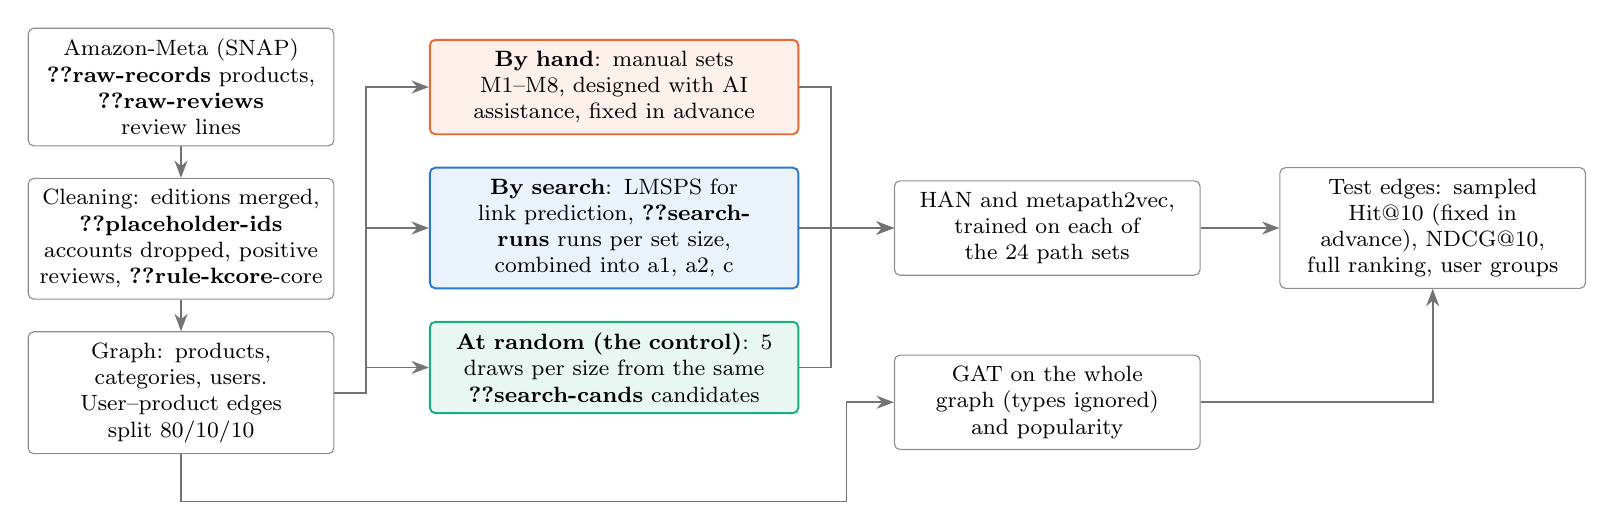
\begin{tikzpicture}[
      font=\footnotesize,
      box/.style={draw=black!45, rounded corners=2pt, align=center, inner sep=4pt,
        text width=#1, minimum height=11mm, execute at begin node={\hyphenpenalty=10000}},
      box/.default=36mm,
      way/.style={box=44mm, draw=#1, fill=#1!10, line width=0.7pt},
      flow/.style={-{Stealth[length=2.2mm]}, black!55, line width=0.6pt}]
    % data
    \node[box] (raw) {Amazon-Meta (SNAP)\\\val{raw-records} products,\\\val{raw-reviews} review lines};
    \node[box, below=4mm of raw] (clean) {Cleaning: editions merged, \val{placeholder-ids} accounts dropped,
      positive reviews, \val{rule-kcore}-core};
    \node[box, below=4mm of clean] (graph) {Graph: products, categories, users.
      User--product edges split 80/10/10};
    % three ways to choose the paths
    \node[way=cManual, right=12mm of raw] (hand) {\textbf{By hand}: manual sets M1--M8,
      designed with AI assistance, fixed in advance};
    \node[way=cSearch, below=4mm of hand] (search) {\textbf{By search}: LMSPS for link prediction,
      \val{search-runs} runs per set size, combined into \code{a1}, \code{a2}, \code{c}};
    \node[way=cRandom, below=4mm of search] (random) {\textbf{At random (the control)}: 5 draws per size from
      the same \val{search-cands} candidates};
    % models and test
    \node[box=36mm, right=12mm of search] (models) {HAN and metapath2vec, trained on each of the
      24 path sets};
    \node[box=36mm, right=10mm of models] (test) {Test edges: sampled Hit@10 (fixed in advance),
      NDCG@10, full ranking, user groups};
    \node[box=36mm, below=4mm of models, yshift=-6mm] (refs) {GAT on the whole graph (types
      ignored) and popularity};
    % arrows
    \draw[flow] (raw) -- (clean);
    \draw[flow] (clean) -- (graph);
    \draw[flow] (graph.east) -- ++(4mm,0) |- (hand.west);
    \draw[flow] (graph.east) -- ++(4mm,0) |- (search.west);
    \draw[flow] (graph.east) -- ++(4mm,0) |- (random.west);
    \draw[flow] (hand.east) -- ++(4mm,0) |- (models.west);
    \draw[flow] (search.east) -- (models.west);
    \draw[flow] (random.east) -- ++(4mm,0) |- (models.west);
    \draw[flow] (models) -- (test);
    \draw[flow] (graph.south) -- ++(0,-6mm) -| ([xshift=-6mm]refs.west) -- (refs.west);
    \draw[flow] (refs.east) -| (test.south);
  \end{tikzpicture}}
  \Description{A flow diagram. The Amazon-Meta data is cleaned and turned into a graph. Two boxes (by hand and by search) choose meta-path sets from the same candidates, and a box at random is the control. Every set goes to HAN and metapath2vec. GAT and popularity use the whole graph. All models are tested on the same held-out edges.}
  \caption{The study. From the same candidate paths, HAN's meta-path sets are chosen by hand or by
    search, with random draws as the control. Every set is trained in HAN and metapath2vec and
    tested on the same held-out edges, with GAT and popularity as baselines that use no meta-paths.}
  \label{fig:pipeline}
\end{widefigure}


\section{The data and the graph}
\label{app:graph}

Table~\ref{tab:graph} summarises the graph and the split of Section~\ref*{P-sec:data}. The rest of
this section gives details of the data that Section~\ref*{P-sec:data} leaves out.

\paragraph{Merging editions.} The merge rule joins \val{edition-pairs} pairs into
\val{edition-clusters} clusters of \val{edition-size-min} to \val{edition-size-max} products
(\val{edition-size-two-pct}\% of them pairs), and leaves \val{raw-works} works out of
\val{raw-usable} usable product records. For the later and larger Amazon review data of
\citet{mcauley2015image}, the data's page warns that the raw reviews contain duplicates, and its
de-duplicated files keep \val{mcauley-dedup-reviews} of its \val{mcauley-raw-reviews}
reviews.\footnote{\url{https://cseweb.ucsd.edu/~jmcauley/datasets/amazon/links.html}, read on
5 November 2026.}

\paragraph{Twin products.} A second test looks for products with exactly the same set of
reviewers. It finds \val{twin-products} products in \val{twin-groups} groups, with \val{twin-test} test
edges that have such a twin in training. Leaving them out changes no run's test Hit@10 by more than
\val{twin-maxdiff}.

\paragraph{Title features.} A product's title vector is an LSA vector: TF-IDF over a vocabulary of
\val{title-vocab} tokens, reduced by truncated SVD to \val{title-dim} dimensions. It is non-zero for
\val{title-coverage-pct}\% of the products.

\paragraph{Category links.} Products link to their leaf categories only. Linking every ancestor as
well would give the median product \val{cat-all-median} categories instead of
\val{after-leafcats-med}, put \val{cat-all-largest-pct}\% of the products into one category and make
P--C--P walks \val{cat-pcp-ratio} times as dense. With leaf links, \code{PCP} leaves only
\val{pcp-isolated} products without a neighbour.

% t2_graph.tex -- T2 of the plan: the graph and the split. Numbers from numbers.tex
% (data/AMAZON/meta.json, audit.json, label files; the split rebuilt and checked by make_numbers.py).
\begin{widetable}[htbp]
  \centering
  \small
  \caption{The graph and the split. Every graph the models see holds the training edges only.}
  \label{tab:graph}
  \begin{tabularx}{\linewidth}{@{}lrL@{}}
    \toprule
    Node type & Nodes & Features \\
    \midrule
    Product (P) & \val{after-products} & \val{title-dim}-d LSA of the title (non-zero for
      \val{title-coverage-pct}\%) and the product group: book \val{group-book-pct}\%, music
      \val{group-music-pct}\%, DVD \val{group-dvd-pct}\%, video \val{group-video-pct}\% \\
    Category (C) & \val{after-categories} & \val{cat-vocab}-d multi-hot vector of the name's tokens (all
      zero for \val{after-zerocat-pct}\%) \\
    User (U) & \val{after-users} & \val{user-dim}-d binary vector hashed from the ID. The search, HAN
      and metapath2vec replace it with a free \val{search-hidden}-d vector \\
    \midrule
    Relation & Edges & \\
    \midrule
    P--P, also bought & \val{after-alsobought} & product pairs (\val{rel-pp-rows} directed rows), made
      symmetric \\
    C--C, parent and child & \val{rel-cc} & \\
    P--C, leaf category & \val{rel-pc} & a median of \val{after-leafcats-med} per product \\
    U--P, positive review & \val{rel-up} & split once at random: \val{split-train} training,
      \val{split-val} validation, \val{split-test} test edges (split seed~\val{split-seed}) \\
    \midrule
    \multicolumn{3}{@{}>{\raggedright\arraybackslash}p{\linewidth}@{}}{Training edges per user:
      median \val{train-deg-med}, mean \val{train-deg-mean}, maximum \val{train-deg-max}. Test
      edges by the user's number of training edges: \val{testdeg-d1} (1--5), \val{testdeg-d2}
      (6--20), \val{testdeg-d3} (21 or more) and \val{testdeg-d0} (none). Each validation and
      test edge is ranked against \val{split-negatives} sampled negatives and against all
      products.} \\
    \bottomrule
  \end{tabularx}
\end{widetable}


\section{Changes from the base papers}
\label{app:changes}

Table~\ref{tab:changes} lists what this study changes in the three base methods, and why. Most
changes follow from the task. LMSPS and HAN were built for node classification. Link prediction
needs a score for a user--product pair, a loss over such pairs and (in the search) care that a
training edge does not reach its own features. Other changes make the comparison fair: every path
set meets the same user side, the same settings and the same stopping rule, in HAN and in
metapath2vec alike. The rest make the search's decision reproducible: it scores every set of its
final pool without noise, and many runs are combined into one choice. The base papers' settings
are as they report them. Ours are those of the runs (Section~\ref{app:settings}).

% t6_changes.tex -- T6 of the plan (appendix): what this study changes in the three base methods,
% condensed from the note on the base papers (Sections 3, 5 and 6). The base papers' own settings
% are typed from the papers; this study's settings are \val{} from numbers.tex (run records).
\begin{widetable}[htbp]
  \centering
  \footnotesize
  \renewcommand{\arraystretch}{1.15}
  \caption{What this study changes in LMSPS \citep{li2024longrange}, HAN
    \citep{wang2019heterogeneous} and metapath2vec \citep{dong2017metapath2vec}, and why.}
  \label{tab:changes}
  \begin{tabularx}{\linewidth}{@{}>{\raggedright\arraybackslash}p{0.27\linewidth}
      >{\raggedright\arraybackslash}p{0.34\linewidth}L@{}}
    \toprule
    In the paper & In this study & Why \\
    \midrule
    \multicolumn{3}{@{}l}{\emph{LMSPS}} \\
    node classification, cross-entropy & user-to-product link prediction: BPR on the dot product
      of a product vector and a free \val{search-hidden}-d user vector & the task of this study \\
    every path from the target type to any type, raw features included & \val{search-cands}
      product-to-product paths of 1--\val{search-hops} hops, each merged with its reverse, no
      self-loops & each path must give HAN a product graph \\
    path features from the whole graph & $\alpha$ learned on validation edges. The weight step
      reads user-path features rebuilt without each quarter of the training edges & a training
      edge is also an edge of the graph \\
    $M = 30$ paths sampled from a pool of $V = 60$, 200 epochs, 20 of warm-up (none in the
      released code) & $M = 4$ or 6 from $V = \val{search-pool}$, \val{search-epochs} epochs,
      \val{search-warmup} of warm-up, dropout \val{search-dropout} & the set sizes of the study,
      so that every set of the final pool can be scored \\
    200 sets sampled from the final pool, each scored with fresh Gumbel noise & all
      \val{search-sets} sets scored once, without noise & the noise moved a set's score more than
      the gaps between sets \\
    one search & \val{search-runs} searches per set size, combined by averaged scores with the
      one-standard-error rule and by a vote checked against a shuffled null & one run cannot rank
      its best sets \\
    LMSPS's own network retrained on the chosen paths & no retraining: the sets go to HAN and
      metapath2vec & the question is whether the paths help HAN \\
    \midrule
    \multicolumn{3}{@{}l}{\emph{HAN}} \\
    node classification, cross-entropy & link prediction, BPR. HAN embeds the products, each user is
      a free \val{han-set-hidden}-d vector & every path set gets the same user side \\
    all meta-path neighbours & the \val{han-set-topk} strongest after every hop, symmetric,
      training edges only, a self-loop & unpruned long paths reach most products \\
    each path's attention layer from its own random start. Path weights learned from the first
      epoch & the same start for every path. Weights held equal for \val{han-set-beta-warmup}
      epochs & otherwise one path takes all the weight within a few epochs \\
    learning rate 0.005, L2 0.001, dropout 0.6, 8 heads of 8 dimensions, patience 100 & learning
      rate \val{han-set-lr}, no L2, dropout \val{han-set-feat-drop}, \val{han-set-num-heads} heads
      of \val{han-set-head-dim}, patience \val{han-set-patience}, at most \val{han-set-stage}
      epochs & sized for one \val{env-gpu-mem}~GB GPU \\
    bag-of-words features, 2--3 short symmetric paths & LSA title vector and product group,
      \val{sets-size-min}--\val{sets-size-max} paths of up to \val{sets-hops-max} hops & the data and the sets compared \\
    \midrule
    \multicolumn{3}{@{}l}{\emph{metapath2vec}} \\
    one symmetric path scheme per run & all paths of a set walked together & one embedding per set,
      as for HAN \\
    negatives from the node-frequency distribution & \val{mtv-set-negatives} negatives sampled
      uniformly within the node type & simpler \\
    1,000 walks per node, length 100, window 7, 128 dimensions & \val{mtv-set-walks-per-node} walks
      per node and path, length \val{mtv-set-walk-length}, window \val{mtv-set-window},
      \val{mtv-set-dim} dimensions & cost, the size of HAN's vectors \\
    \midrule
    \multicolumn{3}{@{}l}{\emph{GAT, as a comparison model}} \\
    in the HAN paper, run on each single meta-path & one type-blind GAT on all relations together,
      without meta-paths & the homogeneous comparison of this study \\
    \bottomrule
  \end{tabularx}
\end{widetable}


\section{The search in detail}
\label{app:search}

\paragraph{Agreement between runs.} The runs score different sets because their final pools
differ, but they rank the sets they share alike: two runs' scores on their shared sets have a median
Spearman correlation of \val{search-agree-4} for four paths and \val{search-agree-6} for six, while
one set's score varies by \val{search-noise-4} and \val{search-noise-6} (standard deviation) from
run to run (Section~\ref*{P-sec:fleet}).

\paragraph{The vote against its null.} The vote picks \val{search-vote-4} distinct sets for four
paths, against a median of \val{search-null-med-4} (90\% range
\val{search-null-lo-4}--\val{search-null-hi-4}) in the \val{search-null-fleets} fleets whose scores
are shuffled within each run. For six paths it picks \val{search-vote-6} sets, against
\val{search-null-med-6} (\val{search-null-lo-6}--\val{search-null-hi-6}). Figure~\ref*{P-fig:ties}b
shows both.

\paragraph{Ranks of the paths.} Over the \val{search-runs} runs of each size, the mean $\alpha$
ranks of \code{PUPUP} and \code{PUPPUP} are \val{rank-pupup-4} and \val{rank-puppup-4} of
\val{search-cands} for four paths, and \val{rank-pupup-6} and \val{rank-puppup-6} for six. The
dense category paths that the manual sets use rank low: \code{PCP} at \val{rank-pcp-4} and
\val{rank-pcp-6}, \code{PCCCP} at \val{rank-pcccp-4} and \val{rank-pcccp-6}. Averaged over both
sizes, the near-empty category paths rank \val{kind-empty-rank} and the dense ones
\val{kind-cat-rank} (Figure~\ref*{P-fig:weights}).

\paragraph{The search's tolerance.} With $\delta = \val{search-delta-alt}$ instead of
\val{search-delta}, the vote picks \val{search-vote-alt-4} and \val{search-vote-alt-6} distinct
sets, against shuffled-score medians of \val{search-null-med-alt-4} and
\val{search-null-med-alt-6}, so the runs still agree beyond chance. The averaged scores do not
depend on $\delta$, and so neither do \code{a1} and \code{a2}.

\section{The random draws and the settings}
\label{app:settings}

With one relevant product per ranking, Recall@10 equals Hit@10 and Precision@10 is Hit@10$/10$,
so Section~\ref*{P-sec:setup} reports neither. Table~\ref{tab:random} lists the ten random draws of
Section~\ref*{P-sec:setup}, and Table~\ref{tab:settings} gives every setting of the search and of the
models. Each setting was fixed before the runs and used for every path set
(Section~\ref*{P-sec:setup}). The values are read from the run records and logs: the search's from its
\val{search-runs-total} records (which agree in every setting except the seed and the set size), and
the models' from the commands and the model descriptions in their logs. Every reported run stopped
early: HAN at epochs \val{han-stop-min}--\val{han-stop-max} of the \val{han-set-stage} allowed, GAT
at \val{gat-stop-min}--\val{gat-stop-max} (one seed after a rerun with a higher cap), and
metapath2vec after \val{mtv-stop-min}--\val{mtv-stop-max} passes.

% t3b_random.tex -- the ten random draws of Table 3, moved to the appendix in paper_v2 (C2).
% Paths from numbers.tex (HAN repository, arch.py).
\begin{widetable}[htbp]
  \centering
  \small
  \caption{The ten random draws, drawn uniformly without replacement from the search's
    \val{search-cands} candidates (Section~\ref*{P-sec:setup}).}
  \label{tab:random}
  \begin{tabular}{@{}ll@{}}
    \toprule
    Draw & Paths \\
    \midrule
    4 paths, draw 1 & \texttt{\val{set-r4d1}} \\
    4 paths, draw 2 & \texttt{\val{set-r4d2}} \\
    4 paths, draw 3 & \texttt{\val{set-r4d3}} \\
    4 paths, draw 4 & \texttt{\val{set-r4d4}} \\
    4 paths, draw 5 & \texttt{\val{set-r4d5}} \\
    \addlinespace
    6 paths, draw 1 & \texttt{\val{set-r6d1}} \\
    6 paths, draw 2 & \texttt{\val{set-r6d2}} \\
    6 paths, draw 3 & \texttt{\val{set-r6d3}} \\
    6 paths, draw 4 & \texttt{\val{set-r6d4}} \\
    6 paths, draw 5 & \texttt{\val{set-r6d5}} \\
    \bottomrule
  \end{tabular}
\end{widetable}

% t8_settings.tex -- the settings of the search and of every model (appendix). Values from
% numbers.tex: the search's from its 60 run records, which make_numbers.py checks are alike apart
% from the seed and the set size; the models' from the commands and model prints in their logs.
\begin{widetable}[htbp]
  \centering
  \footnotesize
  \renewcommand{\arraystretch}{1.0}
  \caption{Every setting of the search and of the models, fixed before the runs and used for every
    path set.}
  \label{tab:settings}
  \begin{tabularx}{\linewidth}{@{}>{\raggedright\arraybackslash}p{0.25\linewidth}L@{}}
    \toprule
    Setting & Value \\
    \midrule
    \multicolumn{2}{@{}l}{\emph{The search (LMSPS for link prediction)}} \\
    Candidates & the \val{search-cands-raw} product-to-product paths of 1 to \val{search-hops}
      hops, \val{search-cands} once each is merged with its reverse. No self-loops \\
    Sets and pool & $M = 4$ or 6 paths. Final pool $V = \val{search-pool}$, so all
      \val{search-sets} sets of $M$ paths are scored \\
    Schedule & \val{search-epochs} epochs, the first \val{search-warmup} with the whole pool.
      Gumbel temperature from \val{search-tau-max} down to \val{search-tau-min} \\
    Network & one linear map per path, PReLU, dropout \val{search-dropout} (input dropout
      \val{search-input-drop}). Product and user vectors of \val{search-hidden} dimensions \\
    Optimiser & Adam: learning rate \val{search-lr} for the weights and \val{search-alr} for
      $\alpha$, weight decay \val{search-weight-decay}. Batches of \val{search-batch} edges \\
    Leakage controls & $\alpha$ learned on the validation edges. The weight step reads user-path
      features from \val{search-folds} versions, each built without one quarter of the training
      edges \\
    Scoring & every set once without Gumbel noise, by validation BPR against the
      \val{split-negatives} fixed negatives. Tie group within $\delta = \val{search-delta}$ \\
    Runs & \val{search-runs} per set size, seeds 1 to \val{search-runs}. Deterministic GPU
      kernels. Propagated features kept in 16-bit floats on the CPU \\
    \midrule
    \multicolumn{2}{@{}l}{\emph{HAN}} \\
    Graphs & per path, each product's \val{han-set-topk} strongest neighbours by walk count after
      every hop, ties broken at random. Binary, symmetric, a self-loop per product. Training
      edges only \\
    Encoder & \val{han-set-in-dim}-d product features. Per path one graph attention layer of
      \val{han-set-num-heads} heads of \val{han-set-head-dim} dimensions, every path from the same
      initial weights \\
    Path weights & semantic attention with a \val{han-set-sem-dim}-d attention vector and a
      softmax temperature of \val{han-set-semantic-tau}. Weights held equal for the first
      \val{han-set-beta-warmup} epochs \\
    Users & a free \val{han-set-hidden}-d vector per user \\
    Training & dropout \val{han-set-feat-drop} on features and \val{han-set-attn-drop} on
      attention. Adam, learning rate \val{han-set-lr}, weight decay \val{han-set-weight-decay}.
      Batches of \val{han-set-batch-size} training edges, each with a fresh negative \\
    Stopping & at most \val{han-set-stage} epochs. Stop when validation BPR has not improved by
      more than \val{han-set-min-delta} for \val{han-set-patience} epochs. Test the best
      checkpoint \\
    \midrule
    \multicolumn{2}{@{}l}{\emph{metapath2vec}} \\
    Walks & per product and path, \val{mtv-set-walks-per-node} walks of length
      \val{mtv-set-walk-length}. All paths of a set walked together, each as a repeated template.
      Training edges only \\
    Skip-gram & \val{mtv-set-dim} dimensions, window \val{mtv-set-window},
      \val{mtv-set-negatives} negatives per pair, sampled uniformly from the context node's type \\
    Training & sparse Adam, learning rate \val{mtv-set-lr}. Batches of \val{mtv-set-batch-walks}
      walks \\
    Stopping & at most \val{mtv-set-epochs} passes over the walks. Validation BPR checked
      \val{mtv-set-evals-per-epoch} times per pass. Stop after \val{mtv-set-patience} checks
      without a gain of more than \val{mtv-set-min-delta} \\
    \midrule
    \multicolumn{2}{@{}l}{\emph{GAT}} \\
    Encoder & one linear projection per node type to \val{gat-set-in-dim} dimensions, then
      \val{gat-set-layers} layers of \val{gat-set-num-heads} heads (\val{gat-set-hidden} dimensions
      in all) on the union of all relations, node types otherwise ignored \\
    Training & dropout \val{gat-set-feat-drop} on features and \val{gat-set-attn-drop} on
      attention. Adam, learning rate \val{gat-set-lr}, weight decay \val{gat-set-weight-decay}.
      Batches of \val{gat-set-batch-size} training edges, whose positive edges are removed from
      the graph the step runs on \\
    Stopping & as HAN, at most \val{gat-cap} epochs. Seed~\val{gat-rerun-seed} reached that cap
      and was rerun with \val{gat-rerun-cap}, stopping at epoch \val{gat-rerun-stop} \\
    \midrule
    \multicolumn{2}{@{}l}{\emph{Popularity}} \\
    Score & the product's number of training users, ties broken at random. One ranking for
      every user \\
    \midrule
    \multicolumn{2}{@{}l}{\emph{Evaluation}} \\
    Split & 80/10/10 at random, split seed~\val{split-seed}, \val{split-negatives} negatives per
      validation and test edge, sampled once \\
    Metrics & sampled Hit@10 (fixed in advance) and NDCG@10. On full ranking, Hit@10 and NDCG@10
      per edge and Recall@20 per user \\
    Seeds & 1 to 3 for the main comparison and GAT, 1 for the other sets \\
    \bottomrule
  \end{tabularx}
\end{widetable}


\section{Full results}
\label{app:full}

Tables~\ref{tab:full-han} and~\ref{tab:full-mtv} give every metric for every path set at seed~1,
the seed that every set was run with. Table~\ref*{P-tab:main} gives the three-seed means of the main
comparison. Across seeds, test Hit@10 of the main runs varies by at most \val{main-hit-sd-max}
(standard deviation, Section~\ref*{P-sec:setup}), so small differences in these tables are within
seed noise.

Table~\ref{tab:groups} gives every model's test Hit@10 by the user's number of training edges
(Section~\ref*{P-sec:res-models}). The rest of this section gives results that
Section~\ref*{P-sec:results} leaves out.

\paragraph{User groups.} HAN's \code{a1} trails the manual set of its size in every user group: by
\val{han-4-hit-d1-diff}, \val{han-4-hit-d2-diff} and \val{han-4-hit-d3-diff} at four paths and by
\val{han-6-hit-d1-diff}, \val{han-6-hit-d2-diff} and \val{han-6-hit-d3-diff} at six, for users with
1--5, 6--20 and 21 or more training edges. GAT's lead over HAN's validation pick is
\val{gat-lead-d1}, \val{gat-lead-d2} and \val{gat-lead-d3} in the same groups.

\paragraph{More paths.} More paths help HAN in every family: the searched sets reach
\val{han-searched6-mean-s1} with six paths against \val{han-searched4-mean-s1} with four, and the
random draws \val{han-r6-hit-mean} against \val{han-r4-hit-mean}.

\paragraph{Path weights and preferences.} HAN gives \code{PUPPUP}, \code{PUPUP} and \code{PUP}
\val{weight-puppup}, \val{weight-pupup} and \val{weight-pup} times an equal share, and it drops
\code{PPCCPP} in all \val{uses-ppccpp} sets that hold it. Over the \val{pref-cand-n} sets drawn from
the candidates, the mean $\alpha$ rank of a set's paths also has a Spearman correlation of
\val{pref-cand-val-rho} with HAN's validation BPR (\val{pref-cand-val-pt}). Among the ten random
draws alone, its correlation with test Hit@10 is weak (\val{pref-random-rho},
\val{pref-random-pt}), and over all 24 sets it is \val{pref-all-rho} (\val{pref-all-pt}): the
relation rests on the searched sets.

\paragraph{HAN and metapath2vec.} The two models prefer different sets: over the 23 sets with a
path through users, their Hit@10 values have a Spearman correlation of only \val{han-mtv-rho}. They
also recommend very different products. In the full-ranking top 10 of \val{bg-users} test users,
HAN's products have a median of \val{bg-han-deg-med} training users
(\val{bg-han-deg-min}--\val{bg-han-deg-max} across the sets). The medians are \val{bg-mtv-deg-med} for
metapath2vec and \val{bg-gat-deg} for GAT, against \val{bg-all-deg} for an average product. Of HAN's
recommendations, \val{bg-han-top1-med}\% come from the 1\% most-bought products, against
\val{bg-gat-top1}\% of GAT's and at most \val{bg-mtv-top1-max}\% of metapath2vec's. By product group, HAN leads
metapath2vec by \val{bg-han-mtv-dvd} on DVDs and \val{bg-han-mtv-video} on videos but trails it on
music (\val{bg-han-mtv-music}, medians over the 23 sets). The two swap places between the sampled
and the full ranking (Section~\ref*{P-sec:res-models}): HAN's popular products win easily against
\val{split-negatives} random negatives, while metapath2vec's long-tail products do relatively better
against all products, the kind of disagreement \citet{krichene2022sampled} warn about.

% t5_groups.tex -- T5 of the plan: every model, overall and by the user's number of training edges
% (results.csv and the run logs, via numbers.tex).
\begin{widetable}[htbp]
  \centering
  \small
  \caption{All models, overall and by the user's number of training edges: test Hit@10, mean
    over the seeds run. GAT, the manual sets and \code{a1} ran with 3 seeds. HAN's validation pick
    (a random draw) and popularity ran with 1 seed. The group sizes are numbers of test edges.}
  \label{tab:groups}
  \begin{tabular*}{\linewidth}{@{\extracolsep{\fill}}lrrrrr@{}}
    \toprule
    & \multicolumn{2}{c}{All test edges} & \multicolumn{3}{c}{User's training edges} \\
    \cmidrule(lr){2-3}\cmidrule(l){4-6}
    Model and set & Sampled & Full & 1--5 & 6--20 & 21 or more \\
    & & & (\val{testdeg-d1}) & (\val{testdeg-d2}) & (\val{testdeg-d3}) \\
    \midrule
    GAT, no meta-paths & \val{gat-hit-mean} & \val{gat-fhit-mean} & \val{gat-hit-d1}
      & \val{gat-hit-d2} & \val{gat-hit-d3} \\
    HAN, validation pick (6 paths, draw 2) & \val{han-r6d2-hit-s1} & \val{han-r6d2-fhit-s1}
      & \val{han-r6d2-hit-d1} & \val{han-r6d2-hit-d2} & \val{han-r6d2-hit-d3} \\
    HAN, M6 & \val{han-m6-hit-mean} & \val{han-m6-fhit-mean} & \val{han-m6-hit-d1}
      & \val{han-m6-hit-d2} & \val{han-m6-hit-d3} \\
    HAN, \code{a1}, 6 paths & \val{han-f6a1-hit-mean} & \val{han-f6a1-fhit-mean}
      & \val{han-f6a1-hit-d1} & \val{han-f6a1-hit-d2} & \val{han-f6a1-hit-d3} \\
    metapath2vec, M5 (validation pick) & \val{mtv-m5-hit-mean} & \val{mtv-m5-fhit-mean}
      & \val{mtv-m5-hit-d1} & \val{mtv-m5-hit-d2} & \val{mtv-m5-hit-d3} \\
    metapath2vec, \code{a1}, 4 paths & \val{mtv-f4a1-hit-mean} & \val{mtv-f4a1-fhit-mean}
      & \val{mtv-f4a1-hit-d1} & \val{mtv-f4a1-hit-d2} & \val{mtv-f4a1-hit-d3} \\
    Popularity & \val{pop-hit} & \val{pop-fhit} & \val{pop-hit-d1} & \val{pop-hit-d2}
      & \val{pop-hit-d3} \\
    \bottomrule
  \end{tabular*}
\end{widetable}

% t9_full.tex -- every path set in HAN and in metapath2vec, every metric, seed 1 (appendix).
% Values from numbers.tex (results.csv): <model>-<set>-<metric>-s1; GAT and popularity as in T4/T5.
% \fullrow{label}{model tag}{set}: one row of six metrics.
\newcommand{\fullrow}[3]{#1 & \val{#2-#3-hit-s1} & \val{#2-#3-ndcg-s1} & \val{#2-#3-fhit-s1}
  & \val{#2-#3-fndcg-s1} & \val{#2-#3-frec-s1} & \val{#2-#3-val-s1} \\}
% \fullbody{model tag}: the 24 sets, by family, as in Table 3.
\newcommand{\fullbody}[1]{%
  \multicolumn{7}{@{}l}{\emph{Searched}} \\
  \fullrow{\code{a1}, 4 paths}{#1}{f4a1}
  \fullrow{\code{a2}, 4 paths}{#1}{f4a2}
  \fullrow{\code{c}, 4 paths}{#1}{f4c}
  \fullrow{\code{a1}, 6 paths}{#1}{f6a1}
  \fullrow{\code{a2}, 6 paths}{#1}{f6a2}
  \fullrow{\code{c}, 6 paths}{#1}{f6c}
  \midrule
  \multicolumn{7}{@{}l}{\emph{Manual}} \\
  \fullrow{M1}{#1}{m1}
  \fullrow{M2}{#1}{m2}
  \fullrow{M3}{#1}{m3}
  \fullrow{M4}{#1}{m4}
  \fullrow{M5}{#1}{m5}
  \fullrow{M6}{#1}{m6}
  \fullrow{M7}{#1}{m7}
  \fullrow{M8}{#1}{m8}
  \midrule
  \multicolumn{7}{@{}l}{\emph{Random}} \\
  \fullrow{4 paths, draw 1}{#1}{r4d1}
  \fullrow{4 paths, draw 2}{#1}{r4d2}
  \fullrow{4 paths, draw 3}{#1}{r4d3}
  \fullrow{4 paths, draw 4}{#1}{r4d4}
  \fullrow{4 paths, draw 5}{#1}{r4d5}
  \fullrow{6 paths, draw 1}{#1}{r6d1}
  \fullrow{6 paths, draw 2}{#1}{r6d2}
  \fullrow{6 paths, draw 3}{#1}{r6d3}
  \fullrow{6 paths, draw 4}{#1}{r6d4}
  \fullrow{6 paths, draw 5}{#1}{r6d5}}
\newcommand{\fullhead}{%
  \toprule
  & \multicolumn{2}{c}{Sampled} & \multicolumn{3}{c}{Full ranking} & \\
  \cmidrule(lr){2-3}\cmidrule(lr){4-6}
  Set & Hit@10 & NDCG@10 & Hit@10 & NDCG@10 & Recall@20 & Val.\ BPR \\
  \midrule}

\begin{widetable}[htbp]
  \centering
  \small
  \caption{HAN on every path set, seed~1 (Table~\ref*{P-tab:main} gives the three-seed means of the
    main comparison). Sampled: each test edge ranked against \val{split-negatives} negatives.
    Full ranking: against every product the user has no edge to, with Recall@20 averaged over
    users. Validation BPR: the loss that early stopping and the validation pick use, lower is
    better. GAT: mean of three seeds. Popularity has no validation loss.}
  \label{tab:full-han}
  \begin{tabular*}{\linewidth}{@{\extracolsep{\fill}}lllllll@{}}
    \fullhead
    \fullbody{han}
    \midrule
    \multicolumn{7}{@{}l}{\emph{Without meta-paths}} \\
    GAT & \val{gat-hit-mean} & \val{gat-ndcg-mean} & \val{gat-fhit-mean} & \val{gat-fndcg-mean}
      & \val{gat-frec-mean} & \val{gat-val-mean} \\
    Popularity & \val{pop-hit} & \val{pop-ndcg} & \val{pop-fhit} & \val{pop-fndcg} & \val{pop-frec}
      & -- \\
    \bottomrule
  \end{tabular*}
\end{widetable}

\begin{widetable}[htbp]
  \centering
  \small
  \caption{metapath2vec on every path set, seed~1. Columns as in Table~\ref{tab:full-han}. M4 has
    no path through users, so its user vectors stay untrained.}
  \label{tab:full-mtv}
  \begin{tabular*}{\linewidth}{@{\extracolsep{\fill}}lllllll@{}}
    \fullhead
    \fullbody{mtv}
    \bottomrule
  \end{tabular*}
\end{widetable}


\section{Reproducibility}
\label{app:repro}

\paragraph{Code.} The data pipeline and the search are in the LMSPS repository, the models and the
evaluation in the HAN repository (the paper's code and data statement). The results in the paper
come from commit \texttt{\val{repo-lmsps-commit}} of the first and commit
\texttt{\val{repo-han-commit}} of the second.

\paragraph{Data.} Amazon-Meta comes from SNAP (Section~\ref*{P-sec:data}). The script
\code{generate_data.bat} in the LMSPS repository (folder \code{hgb}) extracts and cleans the raw
file, writes the graph files and audits the result, with the settings of Section~\ref*{P-sec:data}.
Every run records a fingerprint of its split's training edges (\texttt{\val{split-fingerprint}} for
split seed~\val{split-seed}). The HAN repository's script \code{check_handover.py} confirms that its
data are those the search ran on.

\paragraph{Environment.} One NVIDIA \val{env-gpu} (\val{env-gpu-mem}\,GB) under Windows, with
Python \val{env-python}, PyTorch \val{env-torch} built for CUDA \val{env-cuda} and NumPy
\val{env-numpy}. The search also uses DGL \val{env-dgl}, for its one-time feature propagation on the
CPU. Each repository's \code{requirements.txt} gives its package versions, and the scripts of both
run in one conda environment. The model runs took about \val{models-hours} GPU hours:
\val{han-hours} for the \val{han-runs} HAN runs, \val{mtv-hours} for metapath2vec and
\val{gat-hours} for GAT.

\paragraph{Commands.} In the LMSPS repository (folder \code{hgb}), \code{run_fleet_v3.bat pilot}
first checks that two runs with the same seed agree. Then \code{run_fleet_v3.bat final4} and
\code{final6} run the \val{search-runs} searches of each size, each writing a log and a JSON
record. Finally, \code{run_fleet_v3.bat reselect} combines them into the sets handed over
(Section~\ref*{P-sec:fleet}). In the HAN repository, \code{run_all.bat} runs the experiment in stages:
the data check, the meta-path graphs, two audits, a short memory check, popularity, HAN, GAT,
metapath2vec, the extra seeds and the results table. With the argument \code{dry}, \code{run_all.bat} prints
every command without running it. Section~\ref*{P-sec:setup} gives the run times.

\paragraph{Repeatability.} The search uses deterministic GPU kernels, so the seed decides a run: the
two pilot runs with seed~1 agree in $\alpha$, in the final pool and in all \val{pilot-sets} scored
sets. HAN's training is not bit-for-bit repeatable on the GPU, but the differences are small. A
repeat of one run (\code{a1} with four paths, seed~1) stopped at the same epoch with the same best
epoch (\val{repeat-han-best}), validation BPR (\val{repeat-han-val}) and test Hit@10
(\val{repeat-han-hit}). In the user groups its Hit@10 differed by at most
\val{repeat-han-groupdiff}.

\paragraph{Records.} The LMSPS repository keeps every search's log and record
(\code{hgb/logs/Fleet v3}) with the pilot and the re-selections. The HAN repository keeps every
model run's log and the results table (\code{output/AMAZON/v3}), the logs of the warm-up check
(Section~\ref*{P-sec:res-sensitivity}), and the review notes with their scripts (\code{review}),
among them the output of the check by product group (Section~\ref*{P-sec:res-weights}). The script
\code{paper/make_numbers.py} in the LMSPS repository computes the numbers, tables and figures of
the paper and of this document from these records. It also checks that every run used the same data and that the two
pilot runs agree.

\paragraph{Recommendation tools.} The HAN repository has tools to show what a trained model
recommends. The script \code{recommend.py} lists a user's top products and a product's most
similar ones. The scripts \code{recommend_6path.bat} and \code{recommend_4path.bat} run it on GAT,
and on a representative result of each kind of path set for HAN and for metapath2vec. The script
\code{recommend_api.py} serves the same queries over HTTP.

\paragraph{Not in the repositories.} The repositories do not hold (1) the raw file (which stays
on SNAP's site), (2) the extraction's intermediate files and the graph's node file (which
\code{generate_data.bat} rebuilds) and (3) the trained models (\code{.pt} files), which the check by
product group (Section~\ref*{P-sec:res-weights}) and the recommendation tools need.

% =============================================================================================
\section{Other limitations}
\label{app:limits}

Section~\ref*{P-sec:conclusion} gives the main limitations and sums up two minor ones. Here they are in
detail:
\begin{itemize}
  \item \emph{Training details.} Validation BPR still improved by a median of \val{han-gain-med} in
        the last ten epochs (at most \val{han-gain-max}, and at most \val{searched-gain-max} for
        the searched sets' runs), so longer training would more likely widen the gaps than close
        them. The search chose its sets on validation edges that HAN also uses for early stopping,
        so the sets are compared on test edges only. HAN's user-path graphs contain the training
        edges it learns to predict. The search corrects for this and HAN does not, as the
        correction did not help HAN on a small sample.
  \item \emph{Leaf category links only:} with every ancestor linked, the candidates and the
        search's choices would differ (Section~\ref{app:graph}).
\end{itemize}


\bibliographystyle{ACM-Reference-Format}
\bibliography{references,notes_extra,reading_list}

\end{document}
